% -*- TeX:de -*-
\NeedsTeXFormat{LaTeX2e}
\documentclass[12pt,a4paper]{article}
\usepackage[german]{babel} % german text
\usepackage[DIV12]{typearea} % size of printable area
\usepackage[T1]{fontenc} % font encoding
%\usepackage[latin1]{inputenc} % most likely on Windows
\usepackage[utf8]{inputenc} % probably on Linux
\usepackage{multicol}

% PLOTTING
\usepackage{pgfplots} 
\usepackage{pgfplotstable}
\usepackage{url}
\usepackage{graphicx} % to include images
\usepackage{tikz}
\usepackage{subfigure} % for creating subfigures
\usepackage{amsmath} % a bunch of symbols
\usepackage{amssymb} % even more symbols
\usepackage{booktabs} % pretty tables
\usepackage{makecell} % multi row table heading

% a floating environment for circuits
\usepackage{float}
\usepackage{caption}

%\newfloat{circuit}{tbph}{circuits}
%\floatname{circuit}{Schaltplan}

% a floating environment for diagrams
%\newfloat{diagram}{tbph}{diagrams}
%\floatname{diagram}{Diagramm}

\selectlanguage{german} % use german

\begin{document}

%%%%%%% DECKBLATT %%%%%%%
\thispagestyle{empty}
			\begin{center}
			\Large{Fakultät für Physik}\\
			\end{center}
\begin{verbatim}


\end{verbatim}
							%Eintrag des Wintersemesters
			\begin{center}
			\textbf{\LARGE SS 14}
			\end{center}
\begin{verbatim}


\end{verbatim}
			\begin{center}
			\textbf{\LARGE{Physikalisches Praktikum\\ für das Bachelorstudium}}
			\end{center}
\begin{verbatim}




\end{verbatim}

			\begin{center}
			\textbf{\LARGE{PROTOKOLL}}
			\end{center}
			
\begin{verbatim}

\end{verbatim}

			\begin{flushleft}
			\textbf{\Large{Experiment (Nr., Titel):}}\\
							%Experiment Nr. und Titel statt den Punkten eintragen
			\LARGE{PS04 Spektroskopie und Interferometrie}	
			\end{flushleft}

\begin{verbatim}

\end{verbatim}	
							%Eintragen des Abgabedatums, oder des Erstelldatums des Protokolls
			\begin{flushleft}
			\textbf{\Large{Datum:}} \Large{6.3.2014}
			\end{flushleft}
			
\begin{verbatim}
\end{verbatim}
							%Namen der Protokollschreiber
		\begin{flushleft}
			\textbf{\Large{Namen:}} \Large{Patrick Braun, Johannes Kurz}
			\end{flushleft}

\begin{verbatim}


\end{verbatim}
							%Kurstag und Gruppennummer, zb. Fr/5
			\begin{flushleft}
			\textbf{\Large{Kurstag/Gruppe:}} \Large{DO/4}
			\end{flushleft}

\begin{verbatim}

\end{verbatim}
							%Name des Betreuers, das Praktikum betreute.
			\begin{flushleft}
			\LARGE{\textbf{Betreuer:}}	\Large{Erhard Schafler}	
			\end{flushleft}

%%%%%%% DECKBLATT ENDE %%%%%%%
\pagebreak
\setlength{\columnsep}{20pt}
\begin{multicols}{2}

%%%%%%%%%%%%%%%%%%%%%%%%%%%%%%%%%%%%%%%%%%%%%%%%

%\begin{figure}[H]
%	\centering
%	\includegraphics[scale=0.35]{./figure/beugung.png}
%	\caption{Beugungsmuster Einzelspalt (echtes Foto; schwarz durch weiß ersetzt)}
%	\label{fig:beugungsmuster}
%\end{figure}


%\begin{figure}[H]
%	\centering
%	\pgfplotstabletypeset[
%			columns={abstand, n},
%			col sep=&,
%			columns/abstand/.style={precision=2, zerofill, column name=\makecell{$Abstand$\\$(\pm 0.05)[mm]$} }, 
%			columns/n/.style={column name=\makecell{$n$\\$(Ordnung)$}, precision=0},
%			every head row/.style={before row=\hline,after row=\hline\hline},
%			every last row/.style={after row=\hline},
%			every first column/.style={column type/.add={|}{} },
%			every last column/.style={column type/.add={}{|} }
%			]{
%			abstand & n
%			12.9 & 1
%			24.45 & 2
%			37.40 & 3
%			49.35& 4
%			62.45 & 5
%			74.45 & 6
%			87.45 & 7
%			100.25 & 8
%			
%			}
%	\caption{Messwerte Einzelspalt}
%	\label{tab:werte_einzelspalt}
%\end{figure}



%%%%%%%%%%%%%%%%%%%%%%%%%%%%%%%%%%%%%%%%%%%%%%%%
%%%%%%%%%%%%%%%%%%%%%%%%%%%%%%%%%%%%%%%%%%%%%%%%
\section{Grundlagen, Theorie und Versuchsaufbau}

\subsection{Auflösungsvermögen eines Gitters}
%To DO: Abbildung

In diesem Versuch geht es darum, das Auflösungsvermögen eines Gitters für ein bekanntes Lichtwellenspektrum zu erforschen, und aus dem Setup mit veränderlicher effektiver Gitterbreite die Gitterkonstante $a$ zu ermitteln.\\
In PW8 des Anfängerpraktikums I wurden erstmals die Lichtbeugung und Interferenz am Doppelspalt sowie die Beugung am Gitter untersucht. Durch Messung der unterschiedlichen Beugungswinkel verschiedener scharf abgegrenzter Wellenlängen, wurde aus dem gemessenen Spektrum auf die Art der Lichtquelle, eine Quecksilberdampflampe, geschlossen.\\
Der Aufbau mit Lichtquelle, Fernrohr, Gitter und Beobachtungsfernrohr an einem Goniometer wird auch nun benutzt, um die unbekannte Gitterkonstante zu bestimmen.\\

\begin{figure}[H]
	\centering
	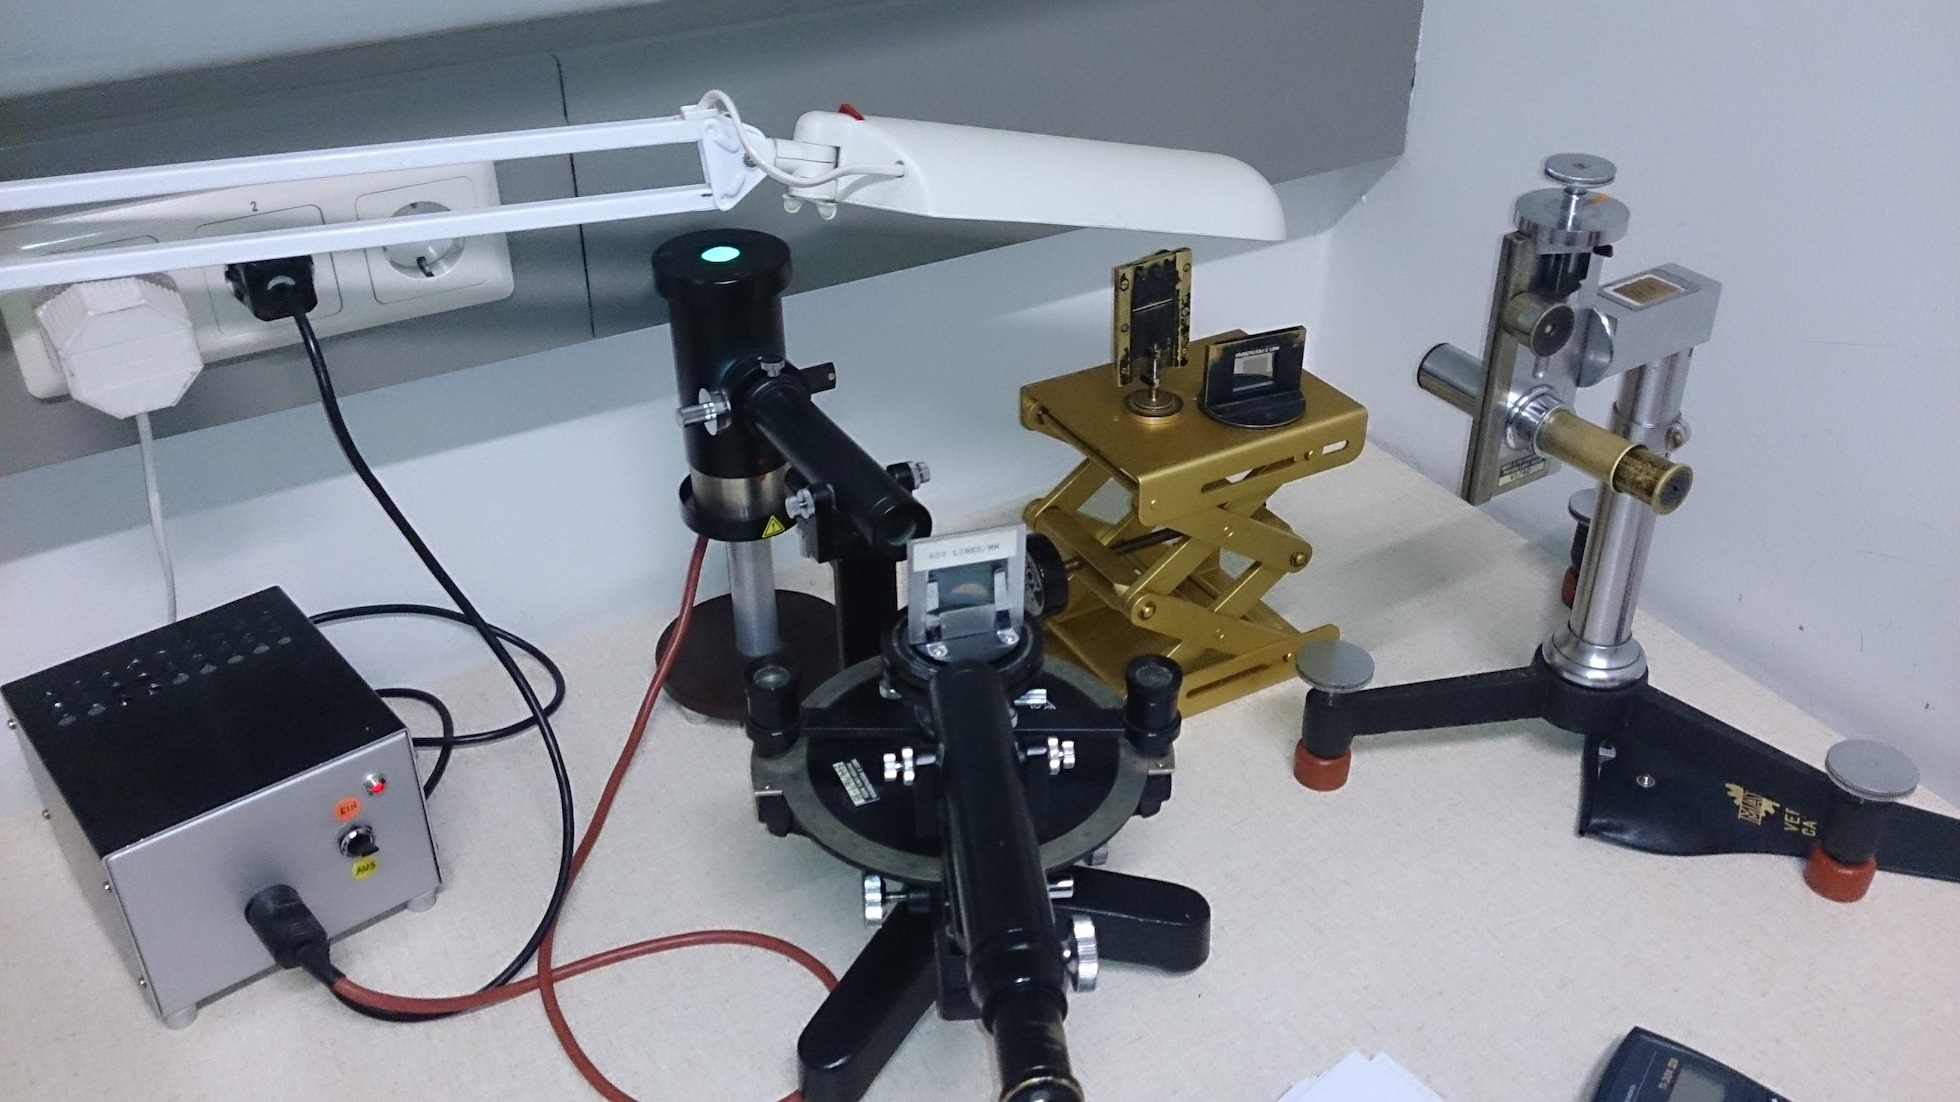
\includegraphics[scale=0.11]{./data/Aufloesungsvermoegen/Aufloesungsvermoegen_Aufbau.jpg}
	\caption{Aufbau mit Lampe, Gitter, Fernrohr und Kathetometer}
	\label{fig:Skizze_Michelson}
\end{figure}



Ausgehend vom Doppelspalt, wird die Ausprägung der Interferenzmaxima bei steigender Spaltanzahl stärker. Werden die Beugungsmaxima am Gitter einzelner Wellenlängen der Hg-Lampe also beobachtet, zeigen sich klar erkennbare deutlich abgegrenzte Linien in den entsprechenden Farben.\\
Verringert man jedoch die Spaltanzahl, indem eine Blende mit variabler Breite vor das Gitter gebracht wird, beginnen die Grenzen der Spektrallinien mit enger werdendem Blendenspalt, zu verschmieren.\\
\\
Da, auch für eine hohe Spaltanzahl ($N \rightarrow \infty $), die Intensitätsmaxima nicht unendlich scharf werden, müssen 2 unterschiedliche Wellenlängen einen gewissen Abstand haben (abhängig von N) um unterscheidbar zu sein (in einem kontinuierlichen Spektrum ist das eben nicht der Fall).\\
Dieses Auflösungsvermögen $A$ ist gegeben durch
$$A= \frac{\lambda}{\Delta \lambda} = n \cdot N$$
wobei $\Delta \lambda$ die Differenz der beiden Wellenlängen ist, und $n$ die Ordnung des Interferenzmaximums.\\
\\
In diesem Versuch wird benutzt, dass das Hg-Spektrum 2 sehr knapp nebeneinanderliegende Wellenlängen im gelben Bereich hat. Sind diese bekannt, lässt sich $A$ berechnen und durch die Ordnungszahl des betrachteten Maximums auch die Spaltanzahl $N$.\\
Die effektiv wirkende Bereich des Gitters ist begrenzt durch die Blendenbreite $B$, deren Betrag gleich N mal der Gitterkonstante a ist: 
$$N=\frac {A}{n}= \frac{\lambda}{\Delta \lambda \cdot n}$$
$$B = a \cdot N$$
$$\Rightarrow a = \frac {B \cdot n}{A}$$

Die Wellenlängen der beiden gelben Linien sind bekannt, aus ihnen wird zunächst A berechnet.\\
Danach wird jeweils ein Beugungsmaximum dieser Doppellinie ausgewählt und die Blende vor dem Gitter so lange verengt, bis die beiden Linien nicht mehr unterscheidbar sind. Es ist also die Grenze des Auflösungsvermögens erreicht.\\
Die Breite der Blende wird anschließend mit einem Kathetometer bestimmt: Das ist ein Fernrohr mit Fadenkreuz, dass durch eine Schraube parallel verschoben werden kann. Zuerst wird eine Seite des Spalts fokussiert, dann an der Schraube gedreht, bis das Fadenkreuz auf die andere Seite zielt. Auf der Skala der Schraube ist die gemessene Breite ablesbar.\\
\\
Die Messung wurde für 3 Ordnungen der Beugungsmaxima jeweils auf beiden Seiten der 0-ten Ordnung gemessen.\\




\subsection{Spektrometrie}
Bei der Spektrometrie [1](2.1.2) versucht man durch Untersuchungen an Absorptions-, Transmissions- und Reflexionsvermögen, Rückschlüsse auf die bestrahlte Materie zu machen. Materie nimmt elektromagnetische Strahlung abhängig von den vorkommenden Elementen unterschiedlich auf. \\
Dringt Licht durch einen Körper verringert sich die Intensität nach dem Lambert-Beer'schen Gesetz wie folgt:

$$I(d) = I(0) * e^{-\alpha *d}$$
I(0)... einfallende Intensität\\
d... Dicke der Probe\\
$\alpha$... Absorptionskoeffizient\\
\\
Der Exponent $A = \alpha * d$ heißt auch Absorbanz bzw. optische Dichte. Die Absorbanz kann auch, einfach umgeformt, durch die Intensitäten beschrieben werden:
$$A = - ln\left( \frac{I(d)}{I(0)} \right)$$
Licht, das durch die Probe hindurchtritt (also nicht absorbiert wird), heißt Transmission und ist durch folgenden Quotienten gegeben:\\
$$T = I_{trans}/I_0$$
Über den Zusammenhang der bisher genannten Größen kann, wie in [1](p. 12), das Reflexionsvermögen definiert werden:
$$R = \frac{(n-1)^2 + k^2}{(n+1)^2 + k^2}$$
Mit diesen Größen lassen sich materialspezifische Spektren errechnen. Um das Hintergrundrauschen des Sensors, sowie vorhandenes Licht und Wärmestrahlung zu eliminieren, werden Messungen mit leeren Proben und schwarzen Objekten vorgenommen. Diese werden dann subtrahiert um eine möglichst rauschfreie Messung zu ermöglichen.\\
\\
Die in PS4 verwendeten Farbfilter sind Plättchen aus Plastik oder Glas, die getönt wurden, also gewisse Farben reflektieren. So können gewisse Wellenlängenbereiche gefiltert werden.\\
Interferenzfilter auf der anderen Seite nützen Interferenz zur Transmission oder Auslöschung von Frequenzen. Zu diesem Zweck werden mehrere Plättchen mit unterschiedlichen Materialien bedampft. Eine Anordnung von $\lambda$/2 und $\lambda$/4 Plättchen führt zur Reflexion bzw. Auslöschung von Frequenzen und zur Verstärkung einer Frequenz. Als Resultat erhält man (fast) monochromatisches Licht.

\subsection{Michelson-Interferometer}

Interferometrie ist eine methode zur Messung von Längen oder Brechungs-indizes.\\
Im vorliegenden Fall wird die Wellenlänge eines Lasers bestimmt.\\
Das Prinzip beruht dabei auf Interferenzerscheinungen durch Laufzeitunterschiede:\\
Der Strahl des Lasers wird durch einen Strahlenteiler in 2 Wege aufgeteilt und wieder zusammengeführt. Bei unterschiedlicher Weglänge ergeben die Laufzeitunterschiede Interferenzerscheinungen.\\
Hier ist ein Weg realisiert durch einen Spiegel in konstantem Abstand vom Strahlenteiler, und einen 2. Spiegel mit veränderlichem Abstand durch eine Mikrometerschraube. Für zusätzliche Genauigkeit wird diese von einem Steuerrad untersetzt angetrieben (siehe Abb.\ref{fig:Skizze_Michelson}).

\begin{figure}[H]
	\centering
	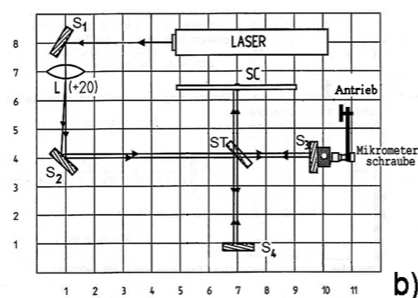
\includegraphics[scale=1.1]{./data/Interferometer/Interferometer_skizze.png}
	\caption{Aufbau-Skizze des Michelson-Interferometers}
	\label{fig:Skizze_Michelson}
\end{figure}

Wird nun der eine Spiegel verschoben ist die Wellenlänge direkt bestimmbar aus dem Quotienten aus dem Wegunterschied und der Anzahl der Maxima bzw. Minima, die durchlaufen werden.\\
Da in diesem Aufbau der Weg vom Strahlenteiler zum verschiebbaren Spiegel und zurück durchlaufen wird, ergibt sich:
$$\lambda = \frac{2\cdot \Delta l}{N}$$
Um genügend große Längen zu messen, und damit die Unsicherheit zu verringern, werden jeweils 100 Minima gezählt und $\Delta l$ auf der Mikrometerschraube abgelesen.\\
Der Antrieb ist durch ein Gummiband mit der Steuerung verbunden, was auch zu einer Dämpfung führt. Der gesamte Aufbau ist dennoch höchst erschütterungsempfindlich und muss bei Bedarf nachkalibriert werden.\\
Da außerdem von Hand durch die Minima durchgeskippt wird und auch die Zählung eine gewisse Konzentration erfordert, ist auch $N$ unsicherheitenbehaftet.



%%%%%%%%%%%%%%%%%%%%%%%%%%%%%%%%%%%%%%%%%%%%%%%%
%%%%%%%%%%%%%%%%%%%%%%%%%%%%%%%%%%%%%%%%%%%%%%%%
\section{Resultate}
\subsection{Auflösungsvermögen eines Gitters}


\begin{figure}[H]
	\centering
	\pgfplotstabletypeset[
			columns={abstand_L, abstand_R, n},
			col sep=&,
			columns/abstand_L/.style={precision=2, zerofill, column name=\makecell{Spaltbreite L\\$(\pm 0.01)$\\$[mm]$} }, 
			columns/abstand_R/.style={precision=2, zerofill, column name=\makecell{Spaltbreite R\\$(\pm 0.01)$\\$[mm]$} }, 
			columns/n/.style={column name=\makecell{$n$\\$(Ordnung)$}},
			every head row/.style={before row=\hline,after row=\hline\hline},
			every last row/.style={after row=\hline},
			every first column/.style={column type/.add={|}{} },
			every last column/.style={column type/.add={}{|} }
			]{
			abstand_L & abstand_R & n
			1.24 & 1.52& 2
			0.79 & 0.87& 3
			0.51 & 0.66 & 4
						
			}
	\caption{Messwerte der Spaltbreite der Blende für linke und rechte Maxima}
	\label{tab:blendenbreite}
\end{figure}



\textbf{Einzelergebnisse:}\\
links:\\
2.Odg.: $a_{2l}=(9.05\pm 0.37) \mu m$\\
3. Odg.: $a_{3l}=(8.65 \pm 0.55) \mu m$\\
4. Odg.: $a_{4l}=(7.45\pm 0.74)\mu m$\\
rechts:\\
2. Odg.: $a_{2r}=(8.62\pm 0.37)\mu m$\\
3. Odg.: $a_{3r}=(9.53\pm 0.55) \mu m$\\
4. Odg.:$a_{4r}=(9.64 \pm 0.74) \mu m$\\
\\
discarded:\\
2.Odg r: $a_{2r-disc.}=(11.10 \pm 0.37)\mu m$\\
\\
\textbf{Mittelwert:}\\
$$a=(8.82 \pm 0.33)\mu m$$




\subsection{Spektrometrie}
Dies sind die gemessenen Spektren von 3 Testflüssigkeiten. Zu vergleichen und identifizieren sind Neodym und Praseodym.

\end{multicols}

\textbf{Flüssigkeit A}

\begin{figure}[H]
	\centering
	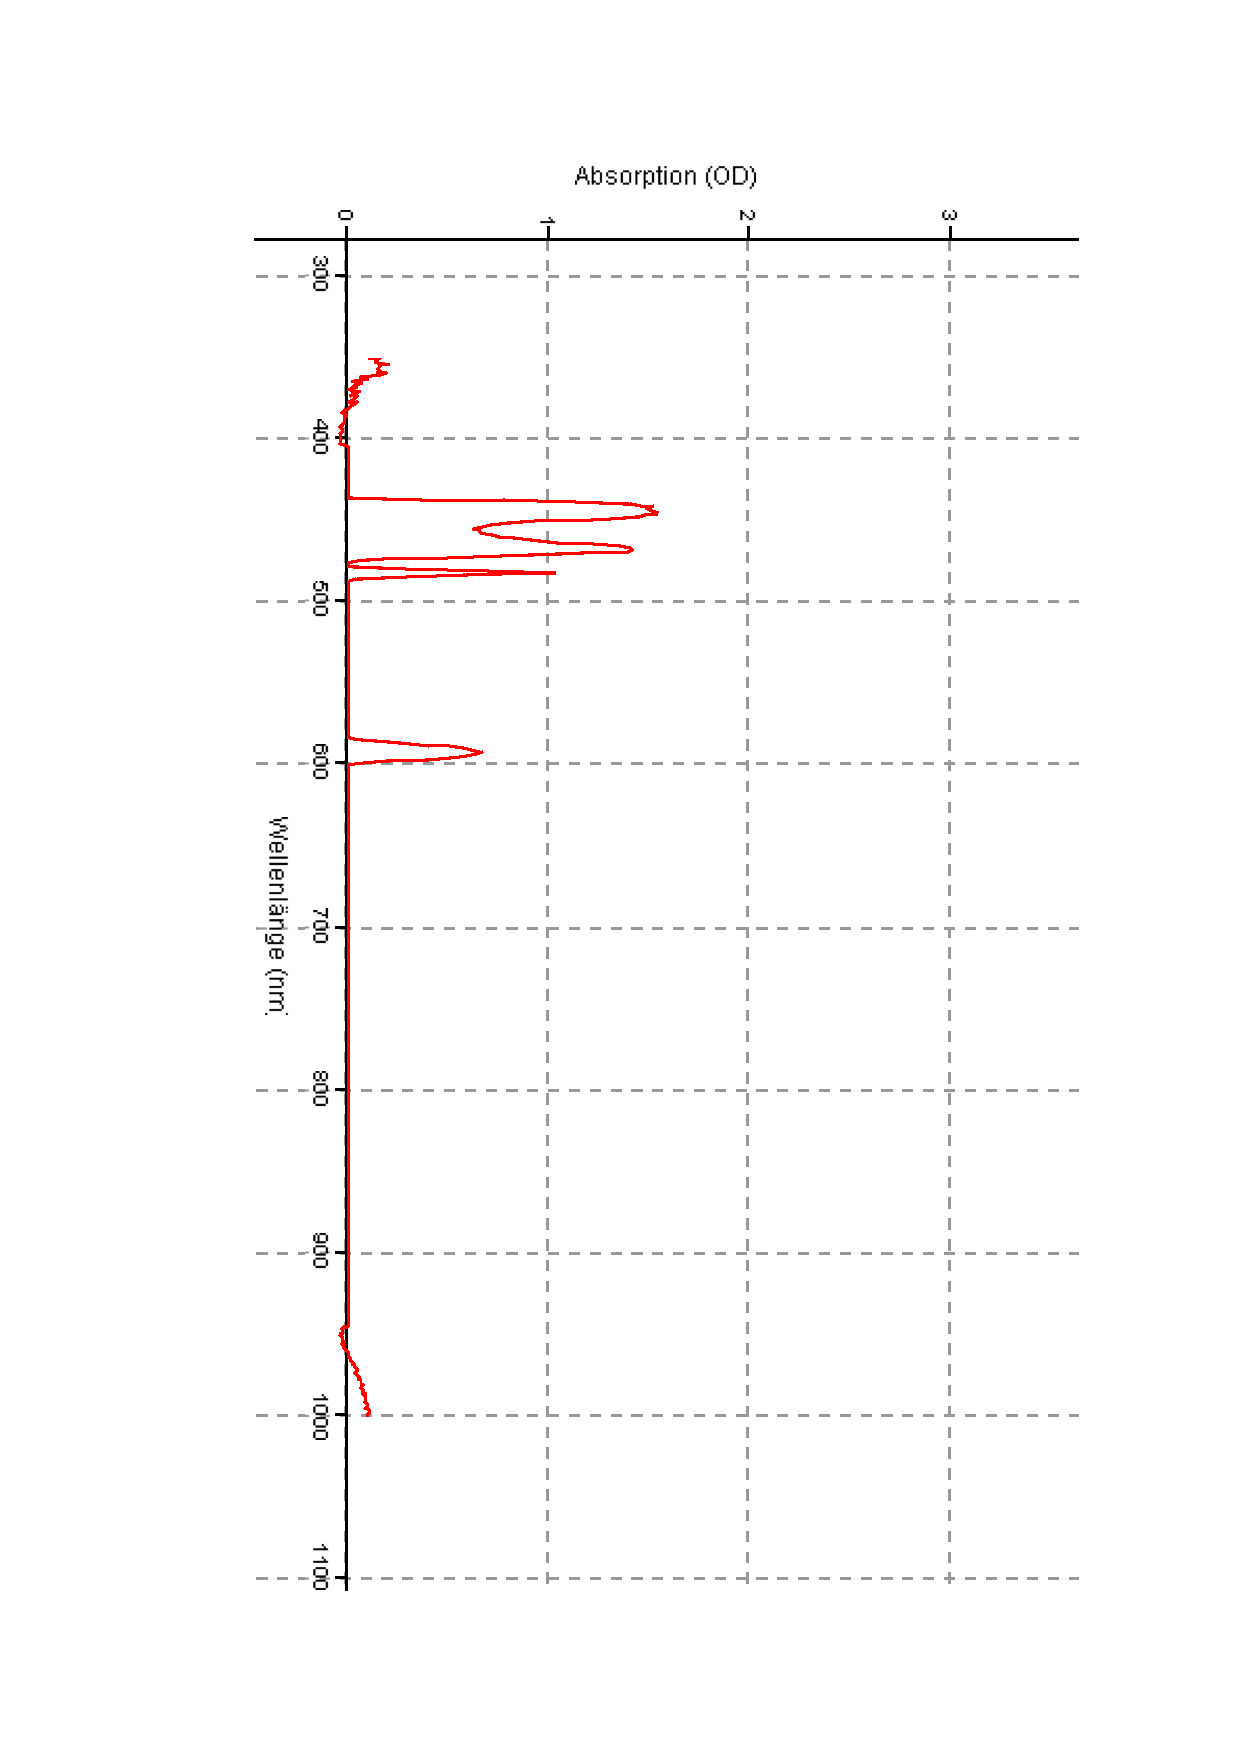
\includegraphics[scale=0.50,angle = 90,trim = 20mm 20mm 20mm 20mm]{./data/Spektro/Absorbtion_A_DO_4.pdf}
	\caption{Absorptionsspektrum von Flüssigkeit A}
	\label{fig:AbsorbtionA}
\end{figure}

\begin{figure}[H]
	\centering
	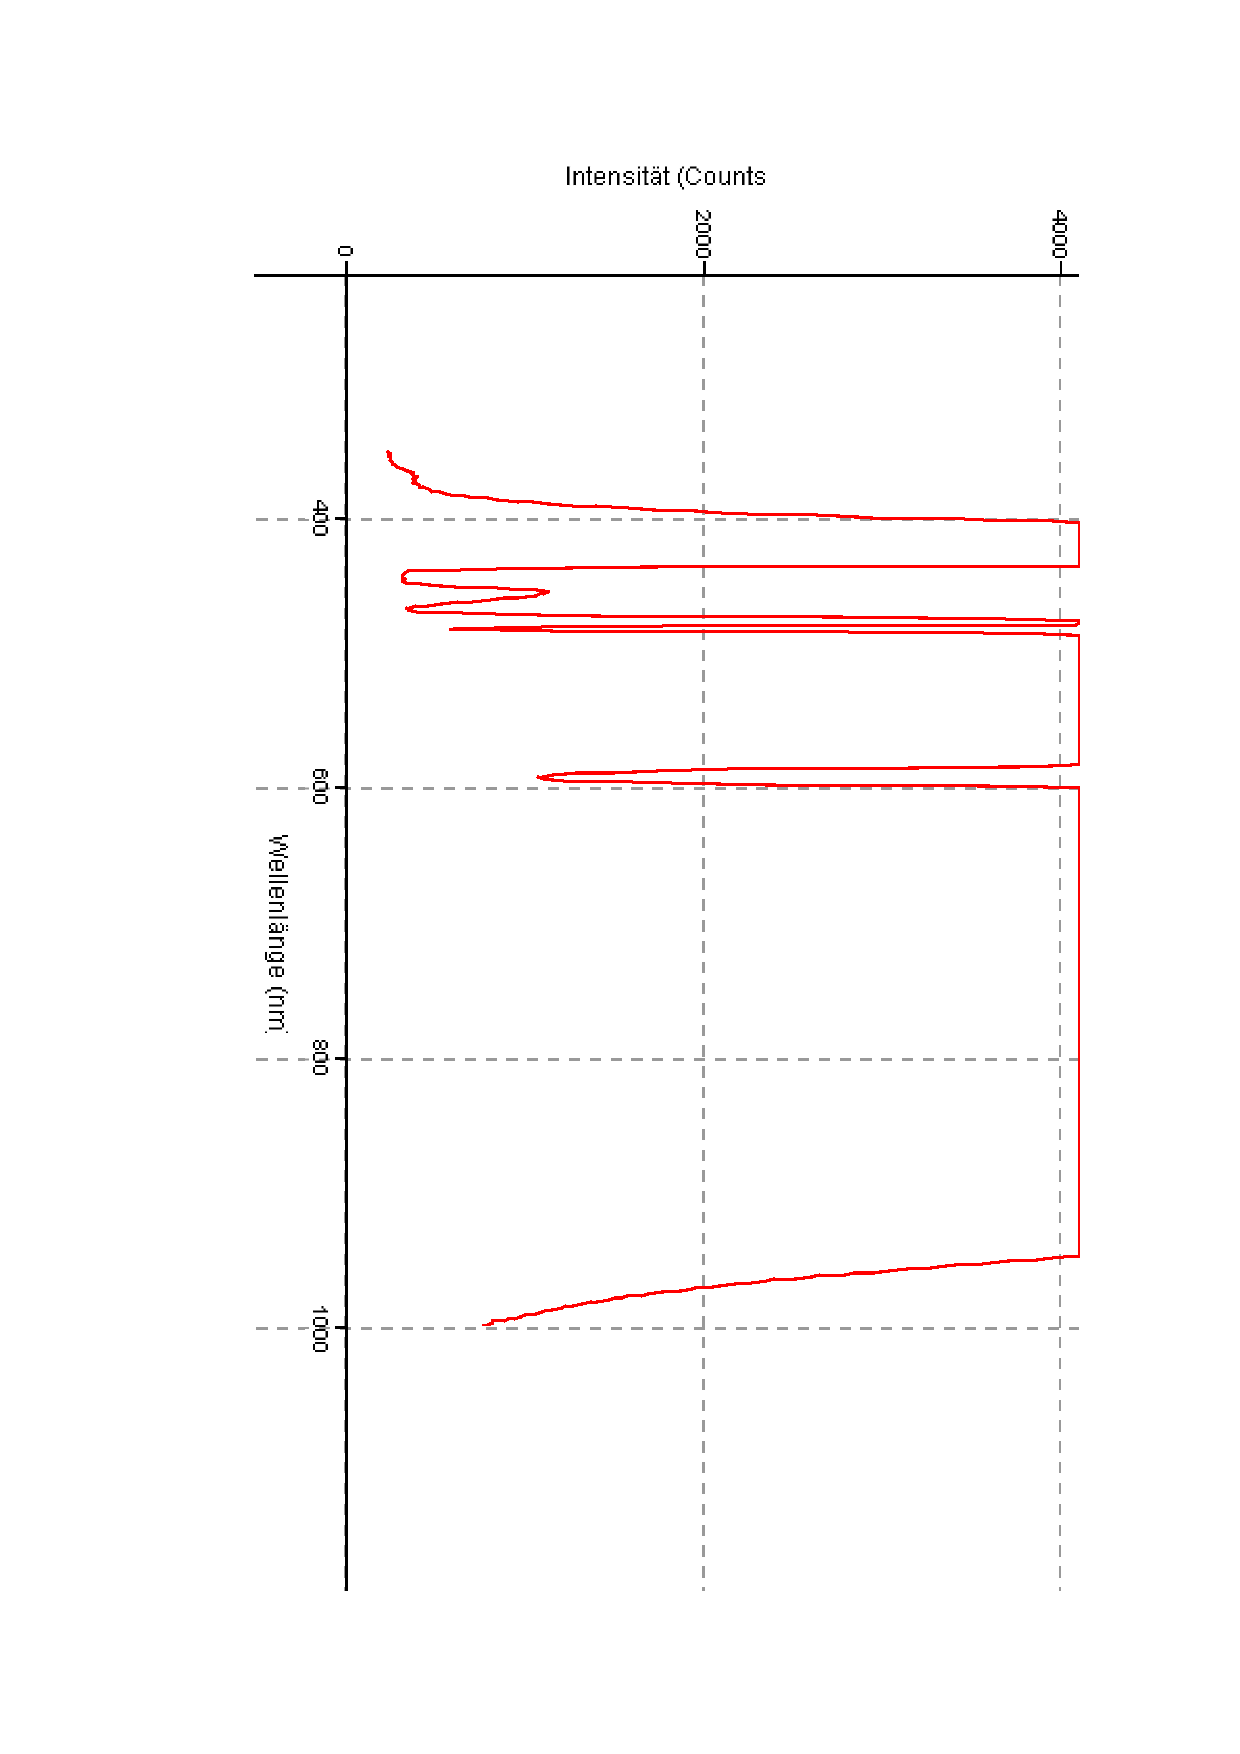
\includegraphics[scale=0.35,angle = 90,trim = 20mm 20mm 20mm 20mm]{./data/Spektro/Transmission_A_DO_4.pdf}
	\caption{Transmissionsspektrum von Flüssigkeit A}
	\label{fig:TransmissionA}
\end{figure}

\textbf{Flüssigkeit B}

\begin{figure}[H]
	\centering
	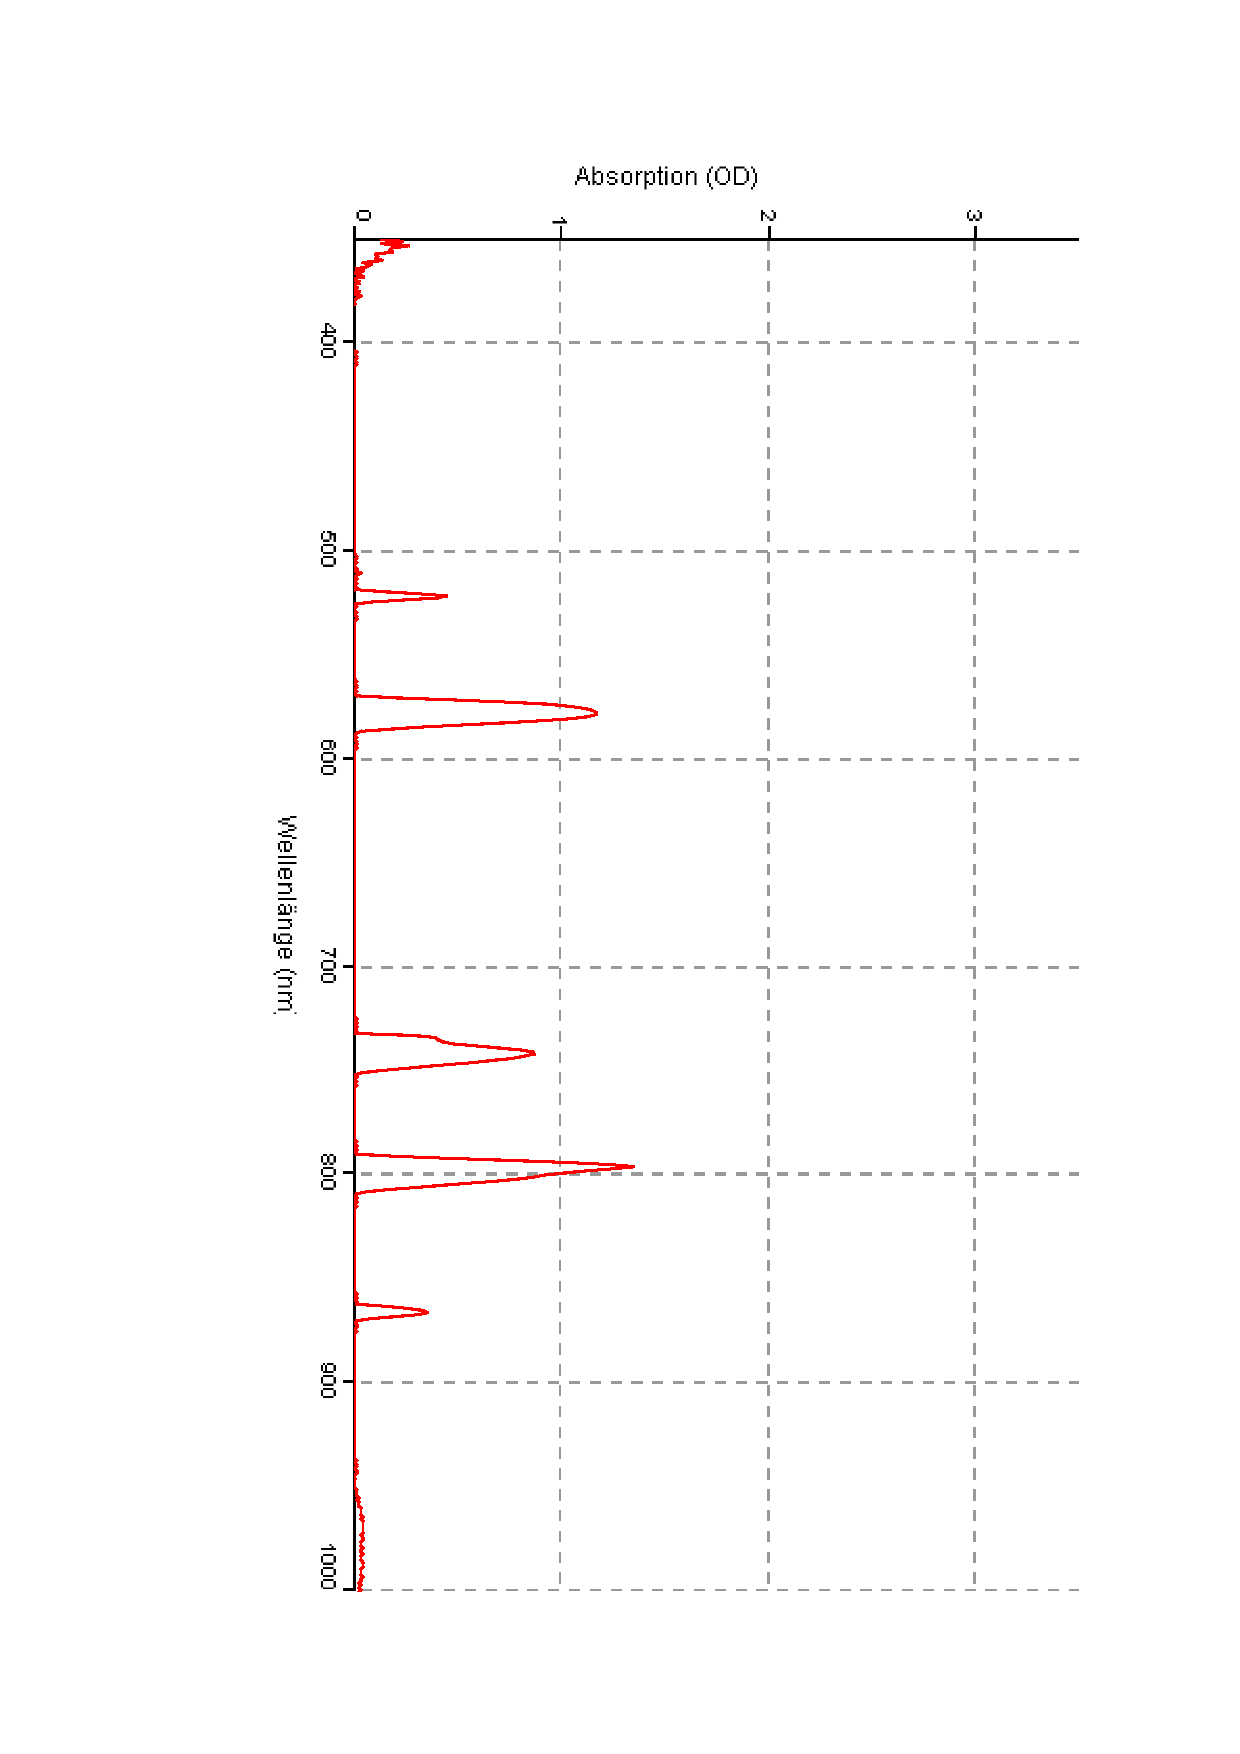
\includegraphics[scale=0.55,angle = 90,trim = 20mm 20mm 20mm 20mm]{./data/Spektro/Absorbtion_B_DO_4.pdf}
	\caption{Absorptionsspektrum von Flüssigkeit B}
	\label{fig:AbsorbtionB}
\end{figure}

\begin{figure}[H]
	\centering
	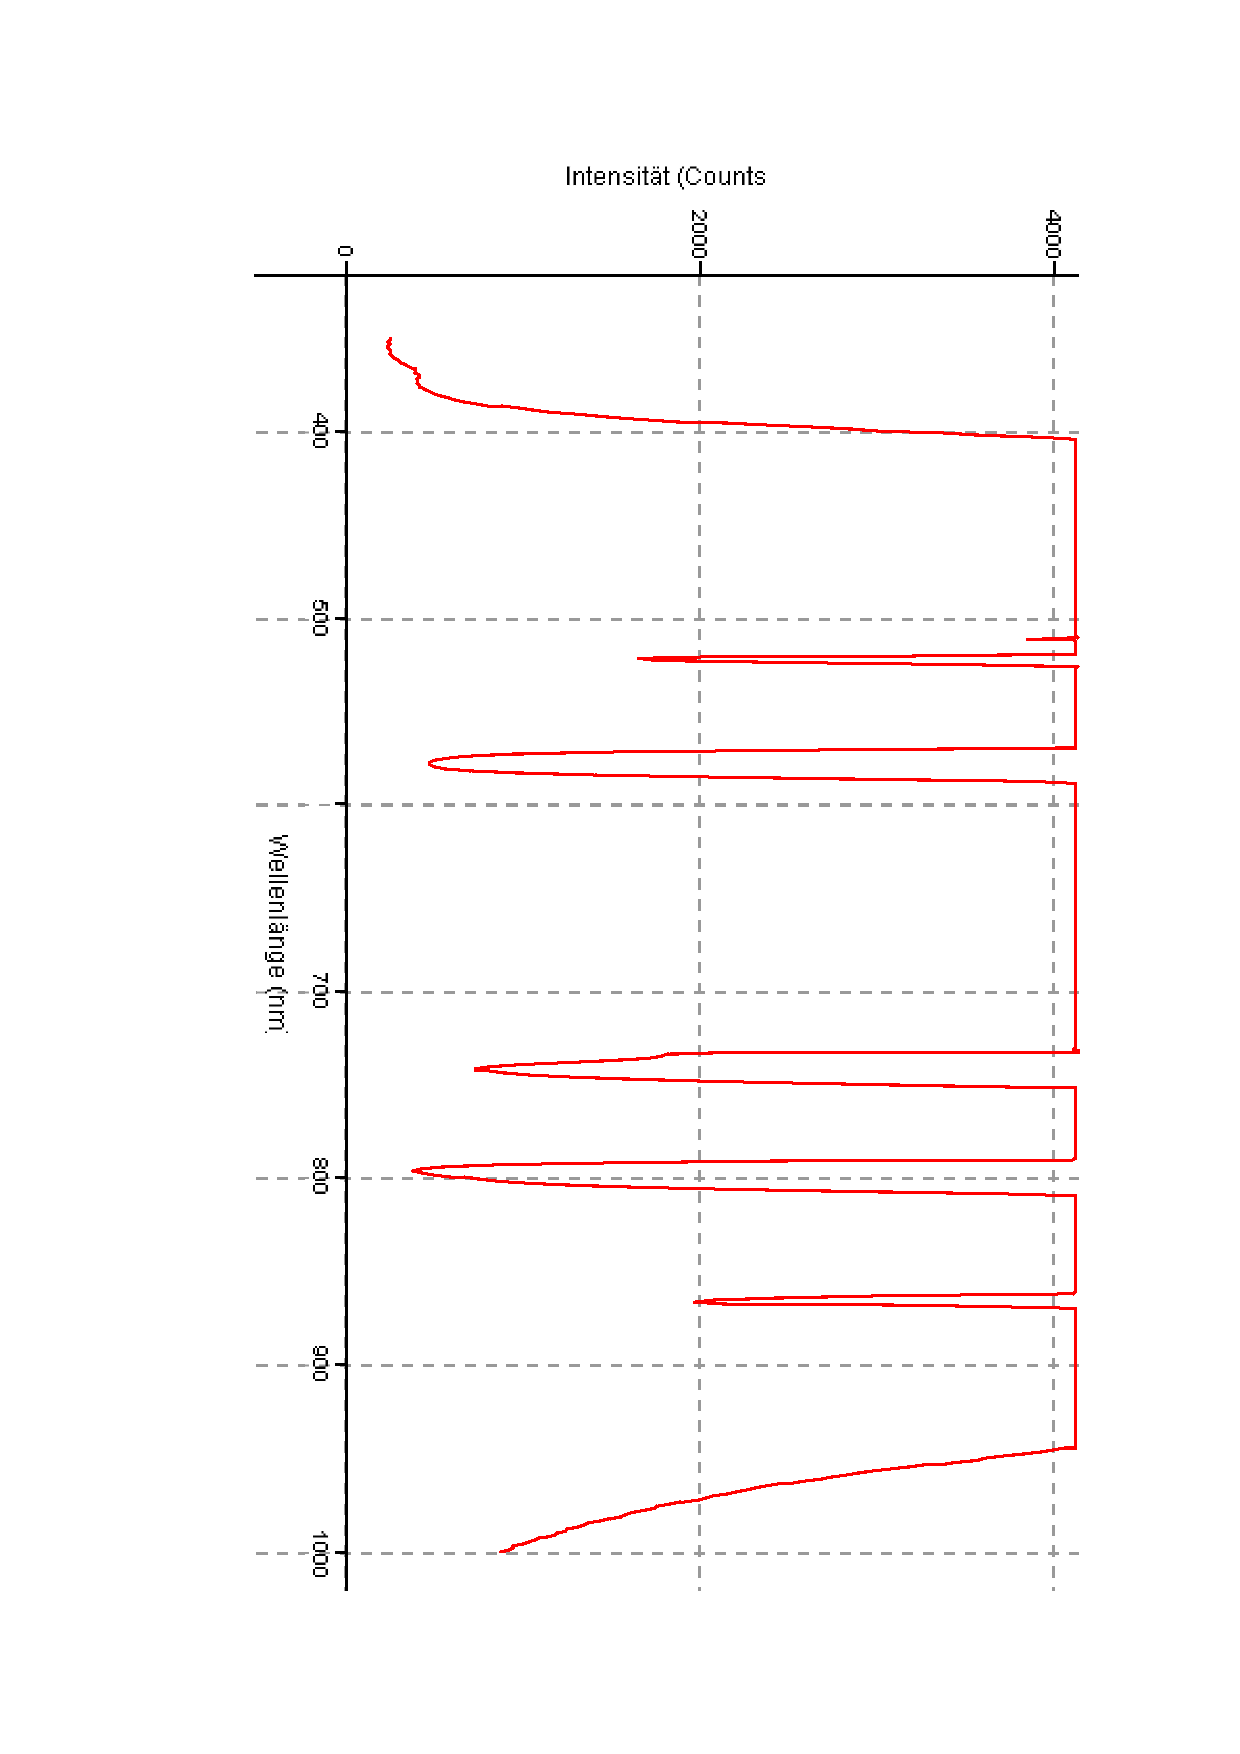
\includegraphics[scale=0.5,angle = 90,trim = 20mm 20mm 20mm 20mm]{./data/Spektro/Transmission_B_DO_4.pdf}
	\caption{Transmissionsspektrum von Flüssigkeit B}
	\label{fig:TransmissionB}
\end{figure}


\pagebreak
\textbf{Flüssigkeit C}

\begin{figure}[H]
	\centering
	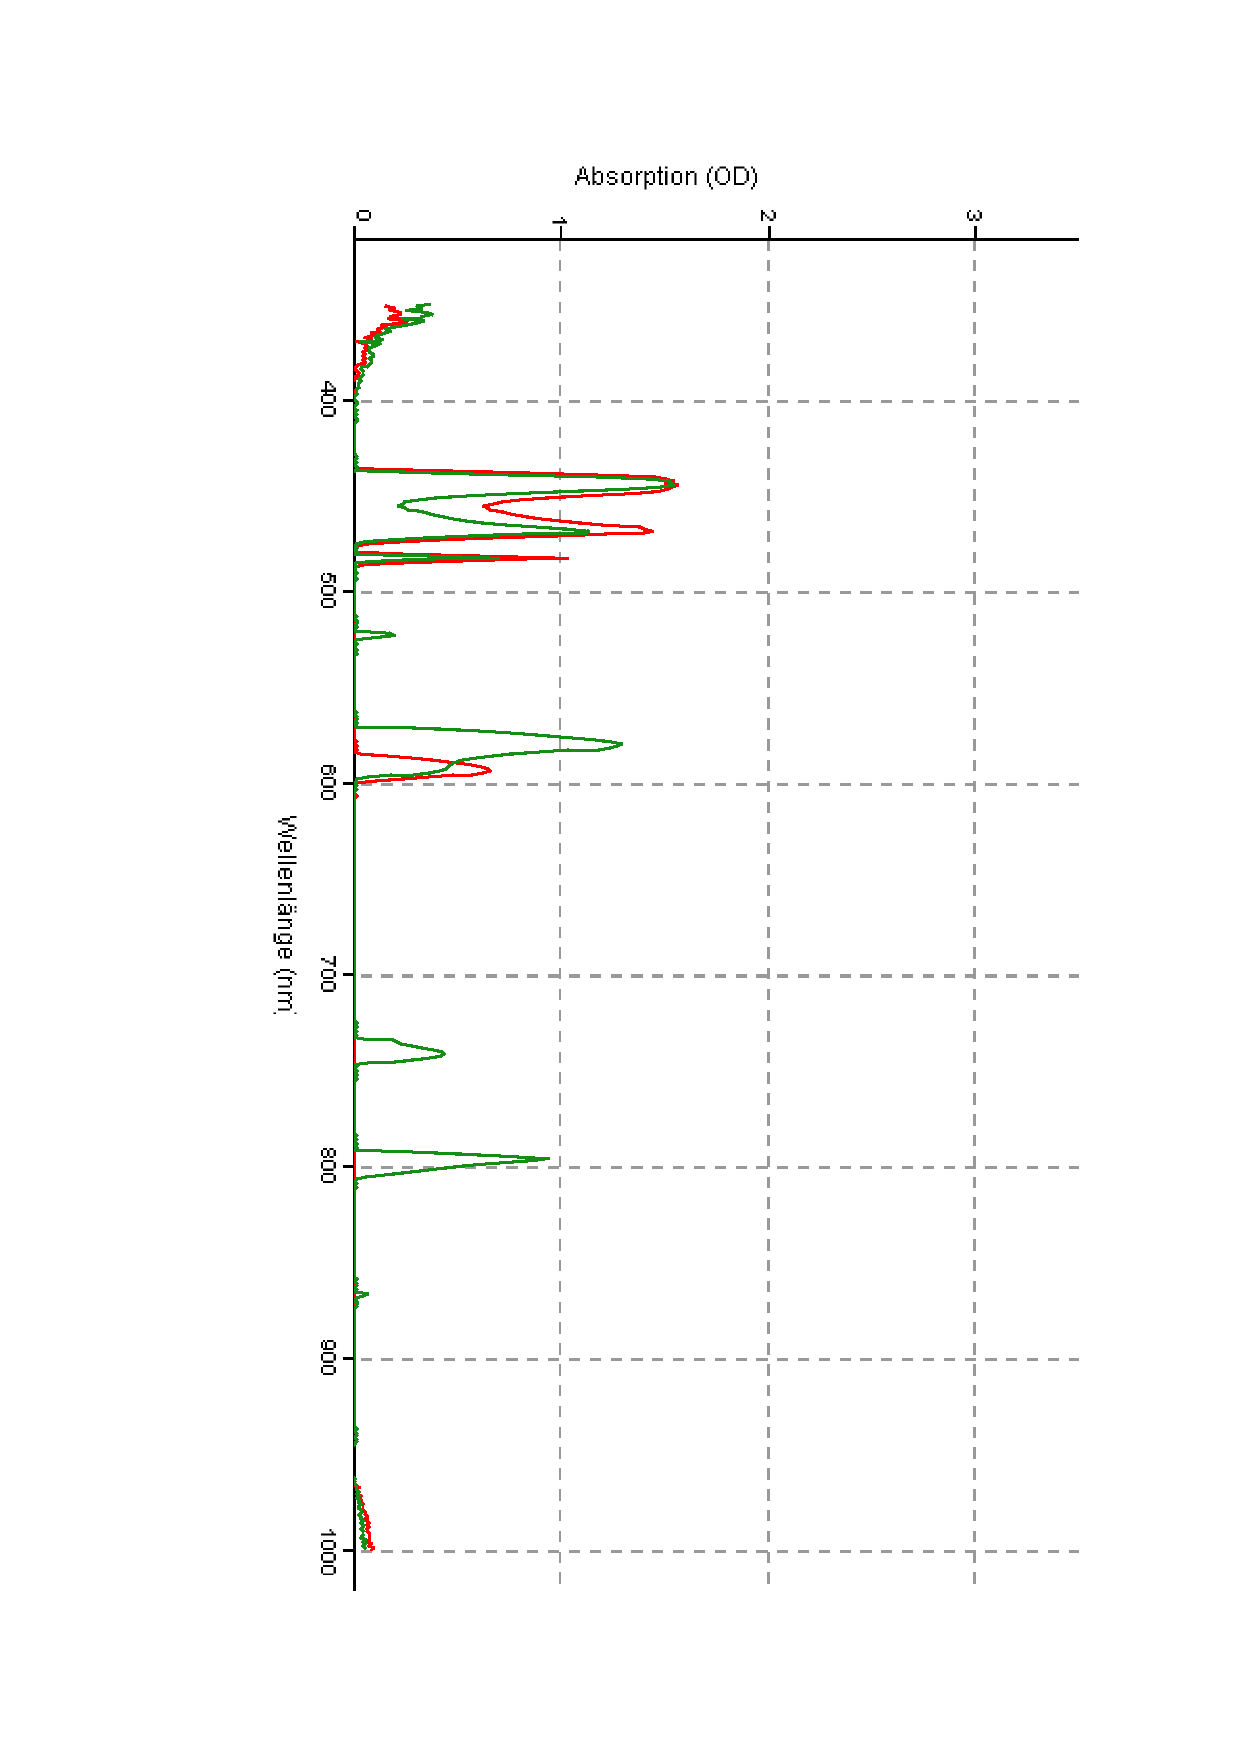
\includegraphics[scale=0.5,angle = 90,trim = 20mm 20mm 20mm 20mm]{./data/Spektro/Absorbtion_CuA_DO_4.pdf}
	\caption{Absorptionsspektrum von Flüssigkeit C über A gelegt}
	\label{fig:AbsorbtionCuA}
\end{figure}

\begin{figure}[H]
	\centering
	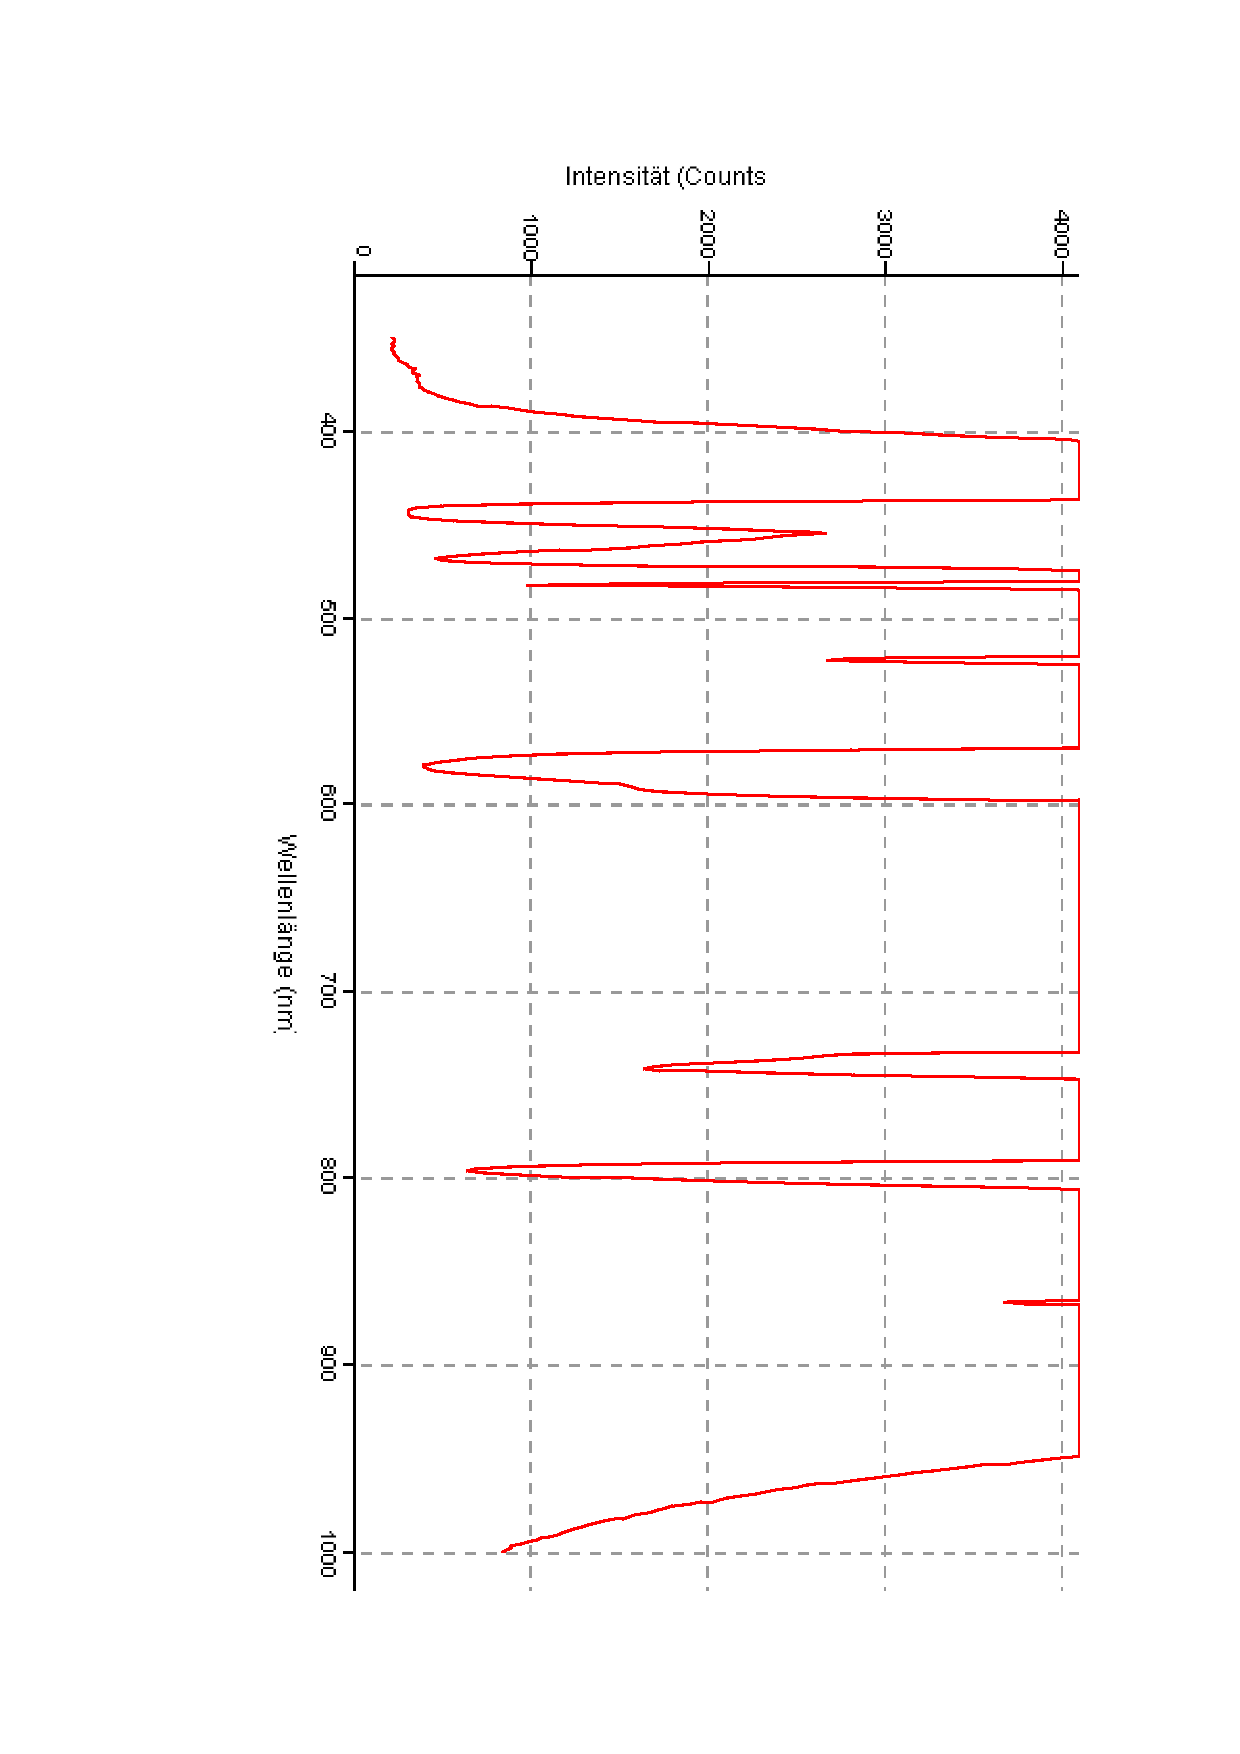
\includegraphics[scale=0.5,angle = 90,trim = 20mm 20mm 20mm 20mm]{./data/Spektro/Transmission_C_DO_4.pdf}
	\caption{Transmissionsspektrum von Flüssigkeit C}
	\label{fig:TransmissionC}
\end{figure}

\begin{figure}[H]
	\centering
	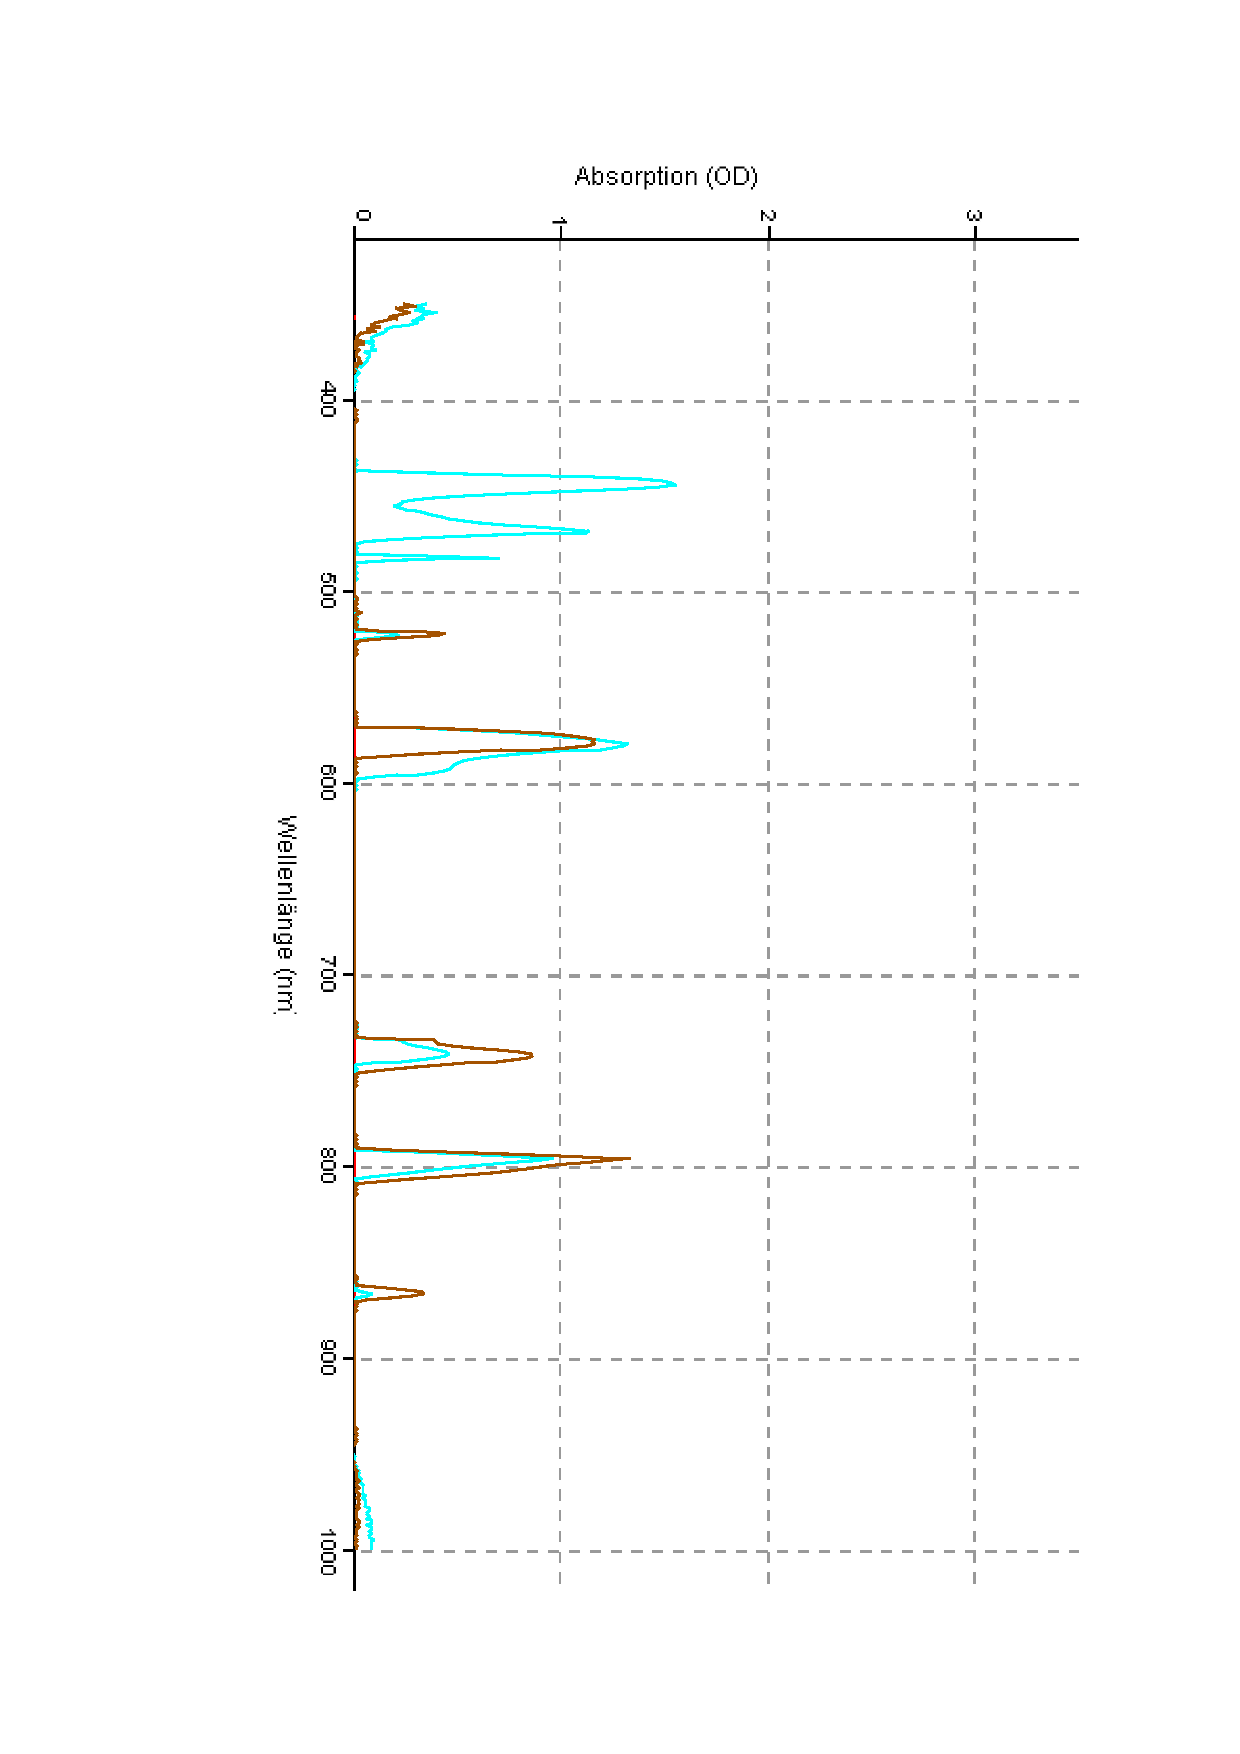
\includegraphics[scale=0.5,angle = 90,trim = 20mm 20mm 20mm 20mm]{./data/Spektro/Absorbtion_CuB_DO_4.pdf}
	\caption{Absorptionsspektrum von Flüssigkeit C über B gelegt}
	\label{fig:AbsorbtionCuB}
\end{figure}

\textbf{Farbfilter}

\begin{figure}[H]
	\centering
	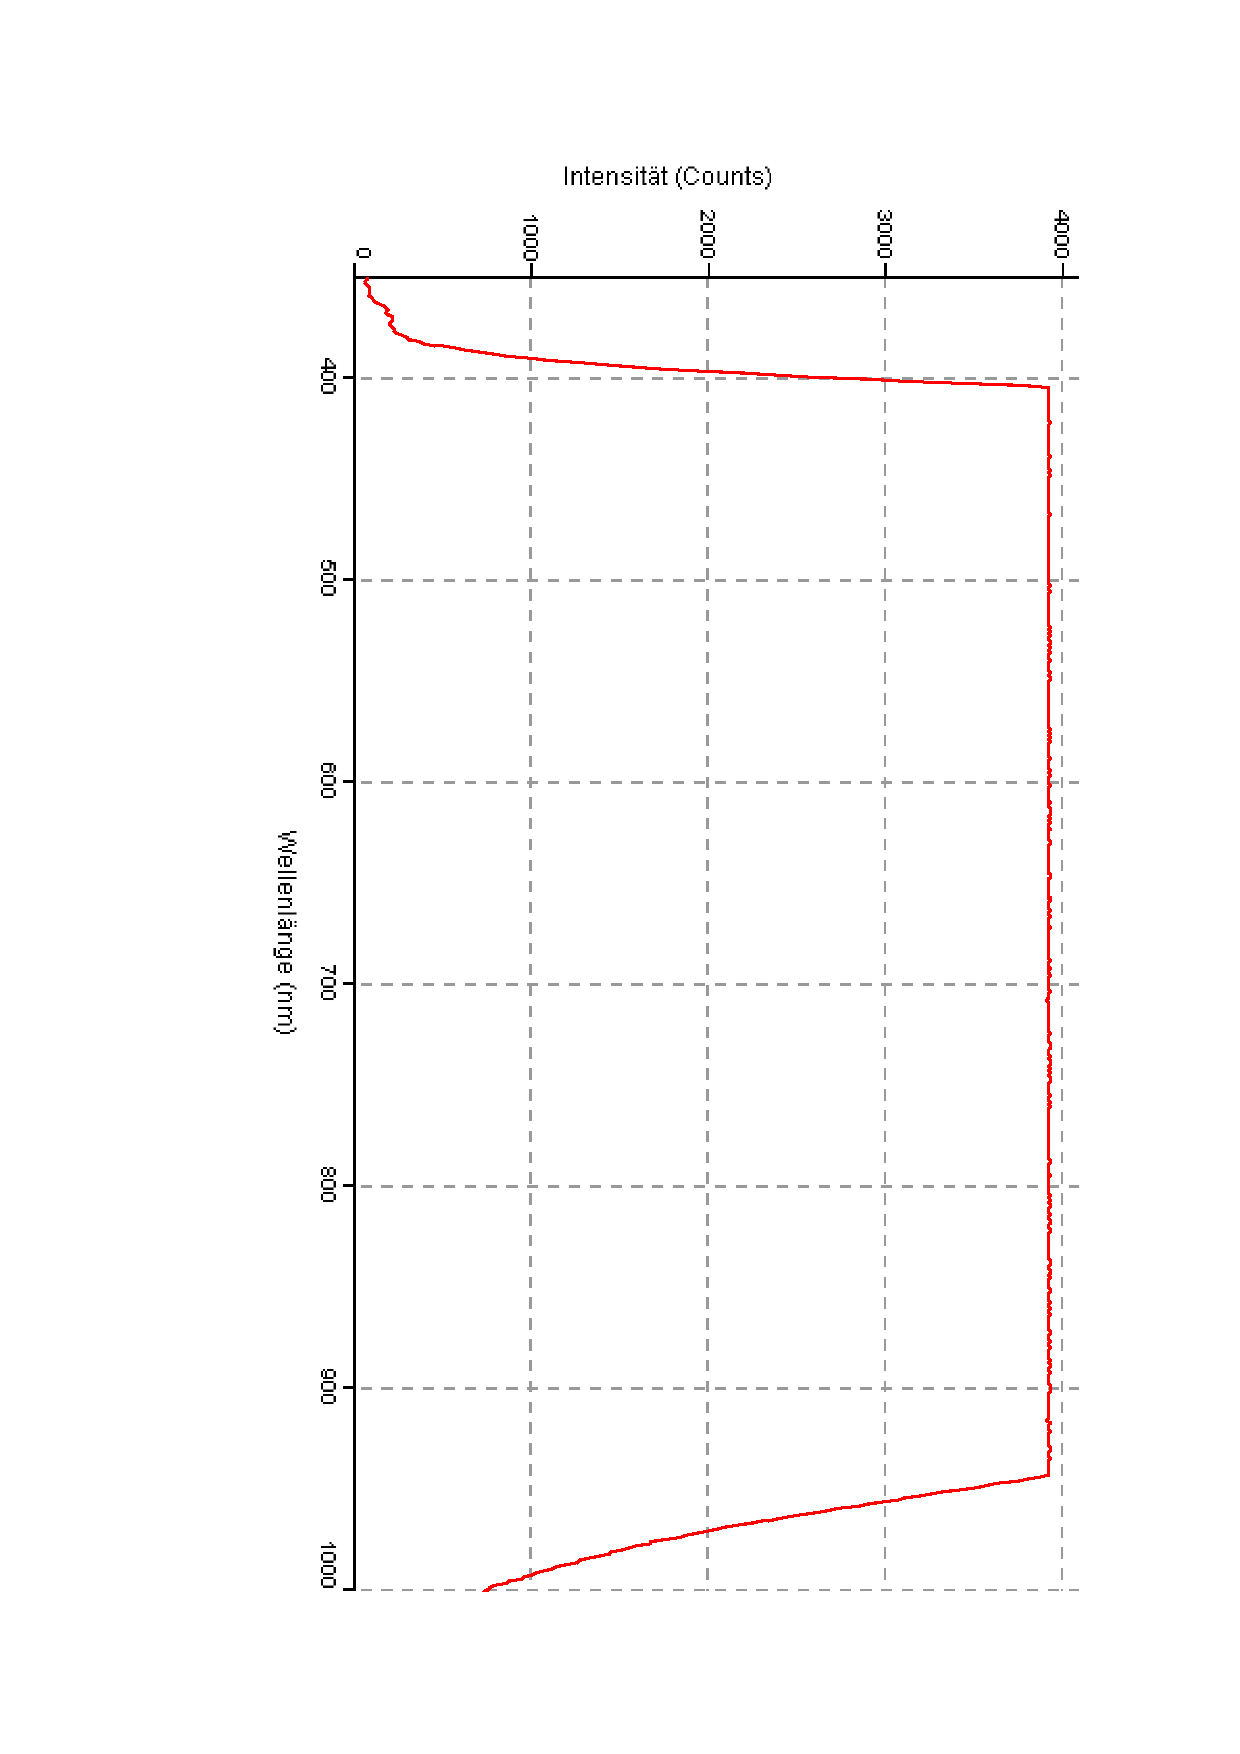
\includegraphics[scale=0.5,angle = 90,trim = 20mm 20mm 20mm 20mm]{./data/Spektro/Dunkel_Leer_DO_4_Kurz_Braun.pdf}
	\caption{Leeres Spektrum ohne Filter}
	\label{fig:FilterOhne}
\end{figure}

\begin{figure}[H]
	\centering
	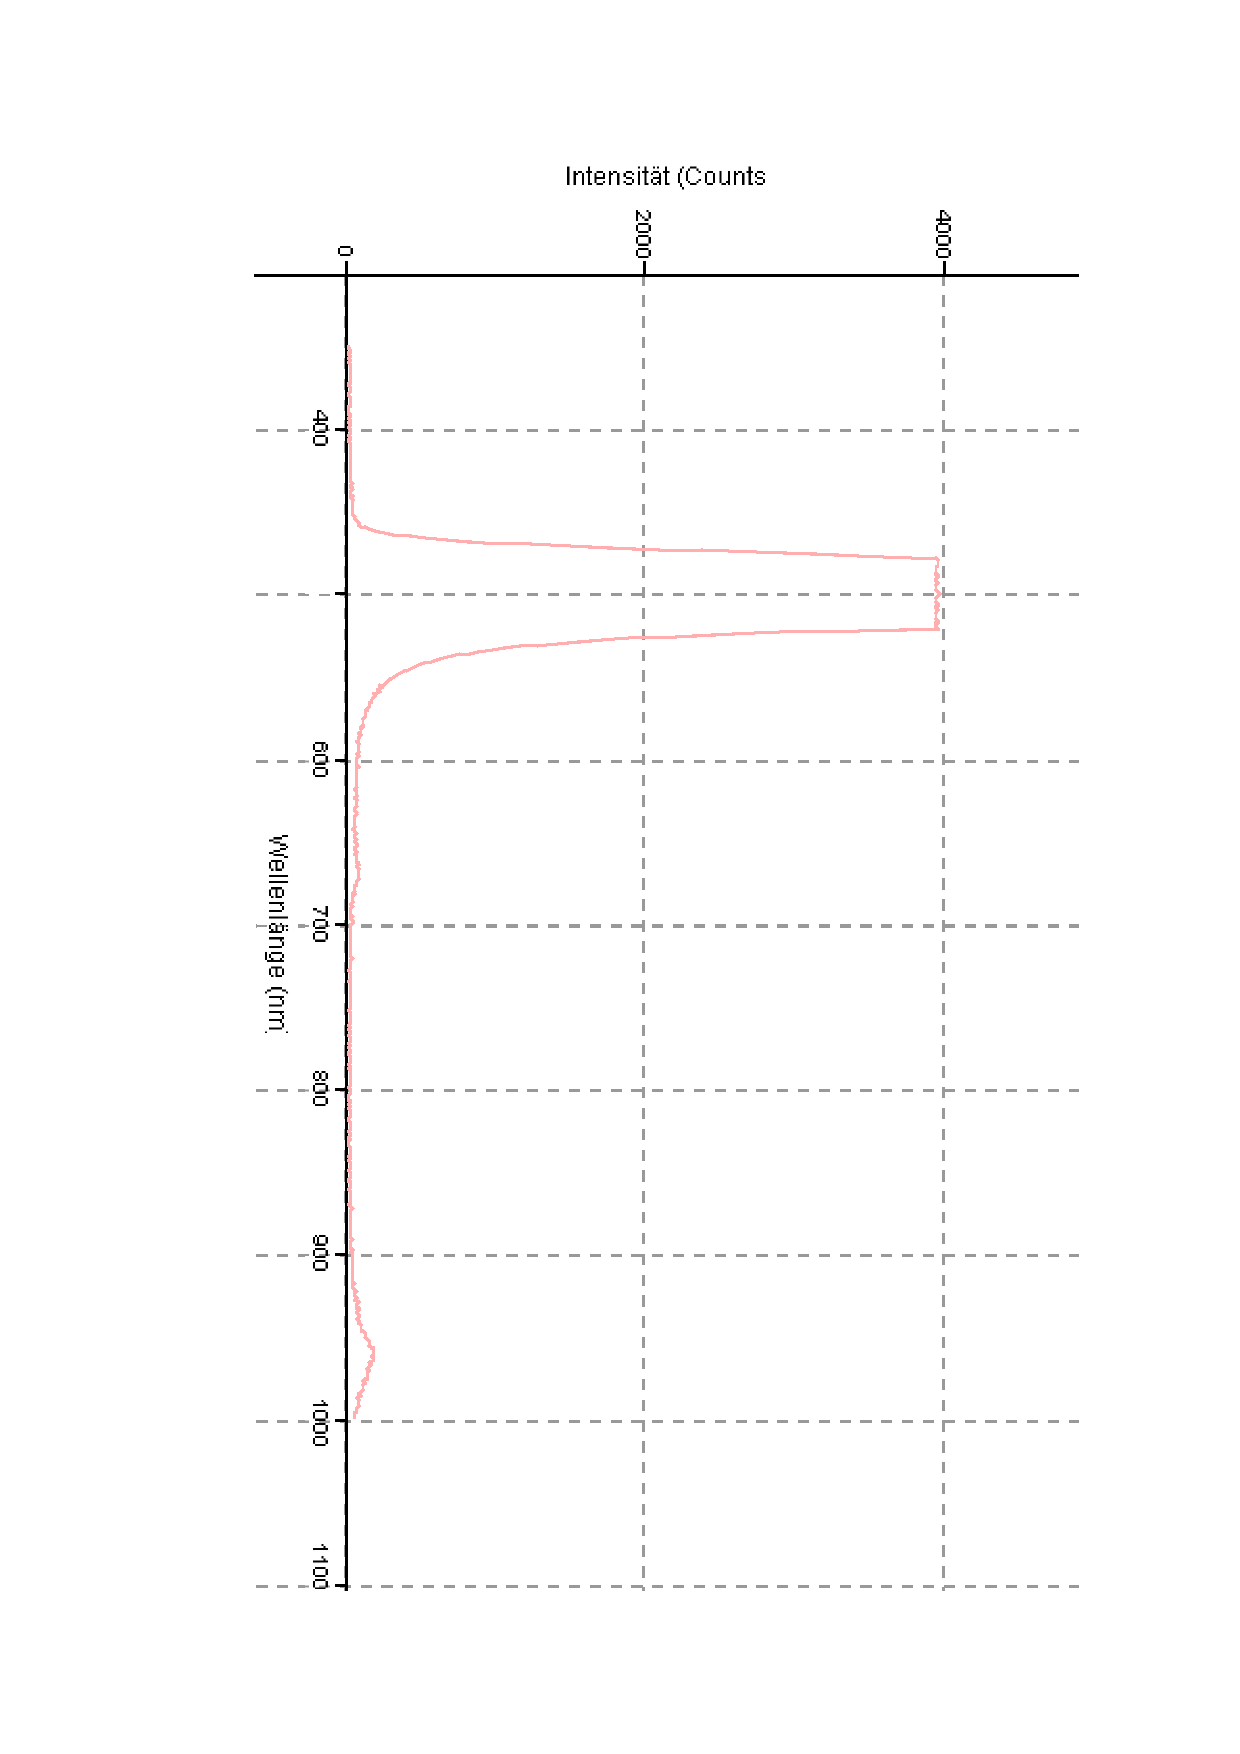
\includegraphics[scale=0.5,angle = 90,trim = 20mm 20mm 20mm 20mm]{./data/Spektro/Farbfilter_Absorbtion_Gruen_DO4.pdf}
	\caption{Spektrum mit grünem Farbfilter}
	\label{fig:FilterGruen}
\end{figure}

\begin{figure}[H]
	\centering
	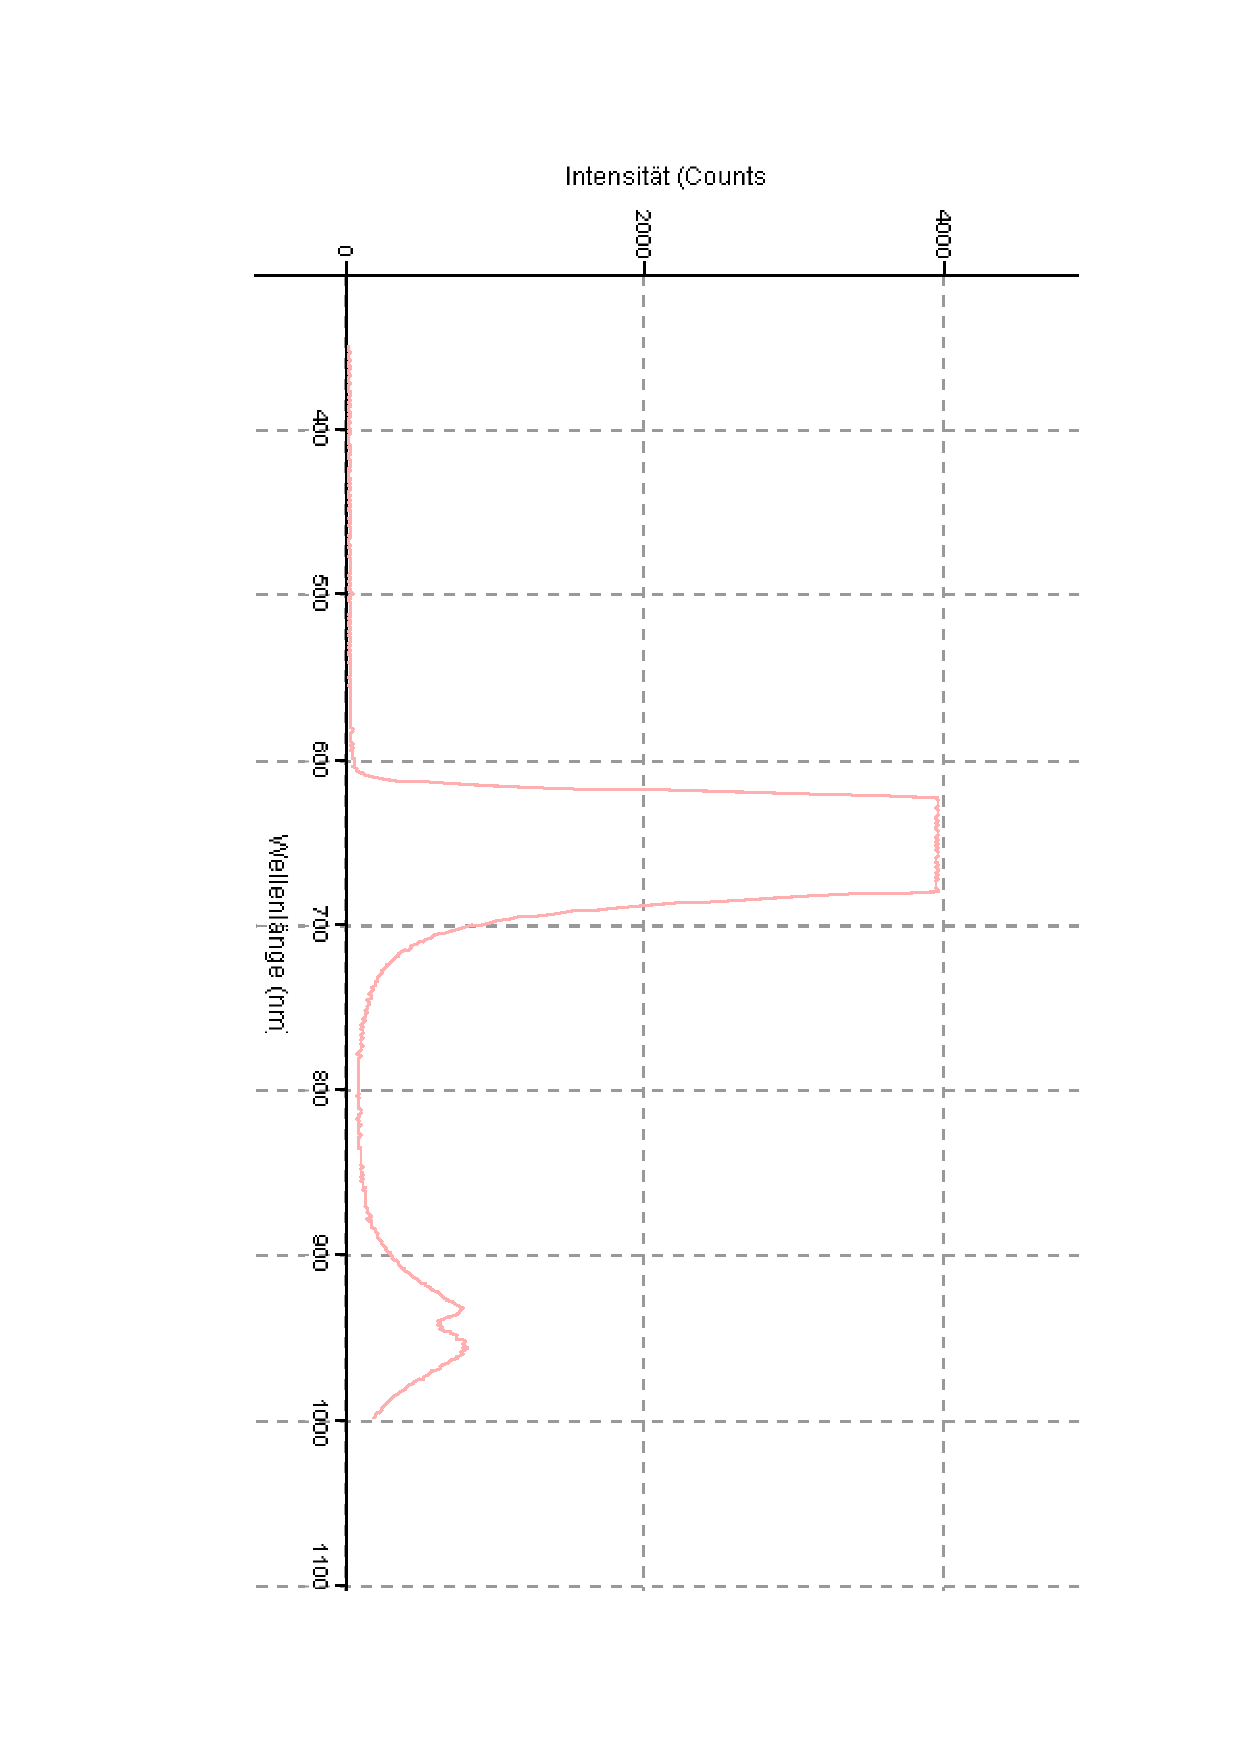
\includegraphics[scale=0.5,angle = 90,trim = 20mm 20mm 20mm 20mm]{./data/Spektro/Farbfilter_Absorbtion_Rot_DO4.pdf}
	\caption{Spektrum mit rotem Farbfilter}
	\label{fig:FilterRot}
\end{figure}

\begin{figure}[H]
	\centering
	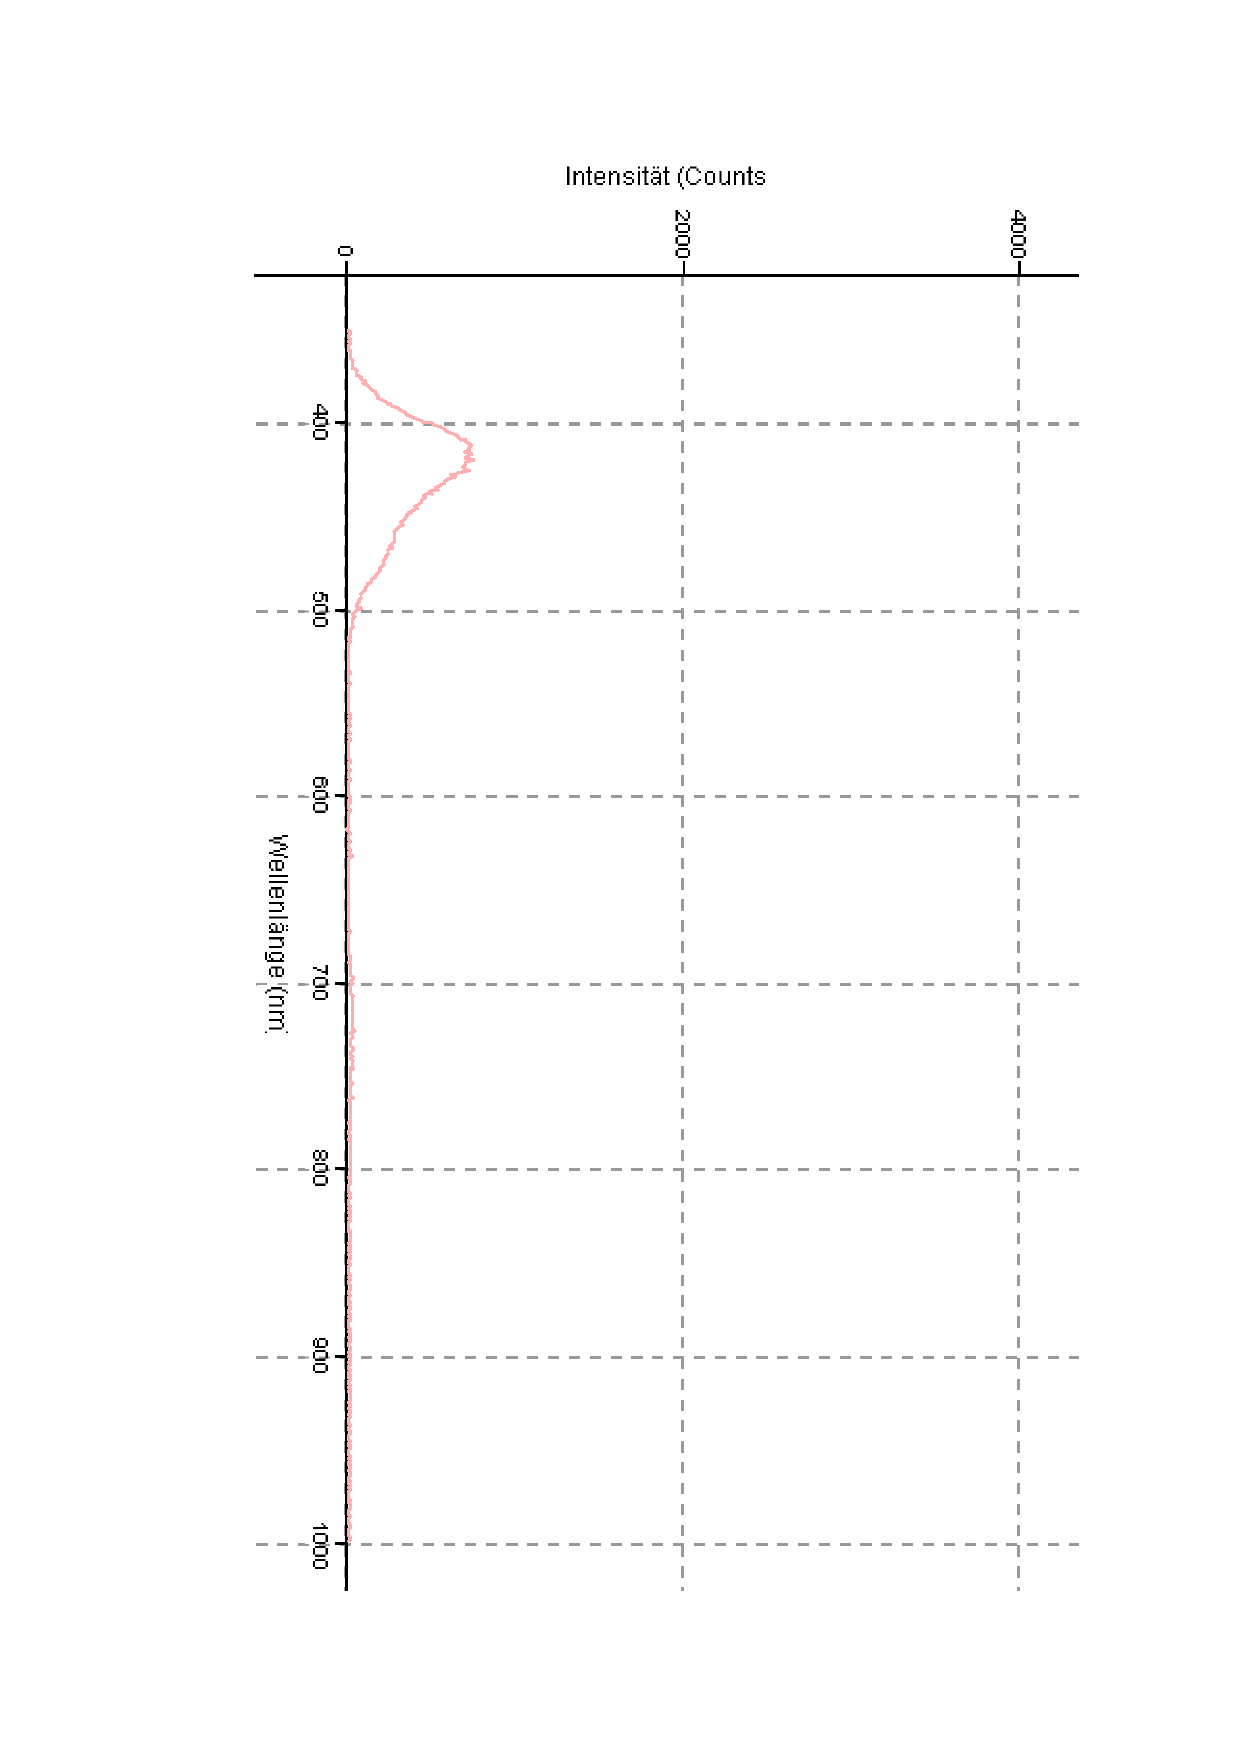
\includegraphics[scale=0.5,angle = 90,trim = 20mm 20mm 20mm 20mm]{./data/Spektro/Farbfilter_Absorbtion_Violett_Blau_DO4.pdf}
	\caption{Spektrum mit violett-blauem Farbfilter}
	\label{fig:FilterBlau}
\end{figure}

\textbf{Interferenzfilter}

\begin{figure}[H]
	\centering
	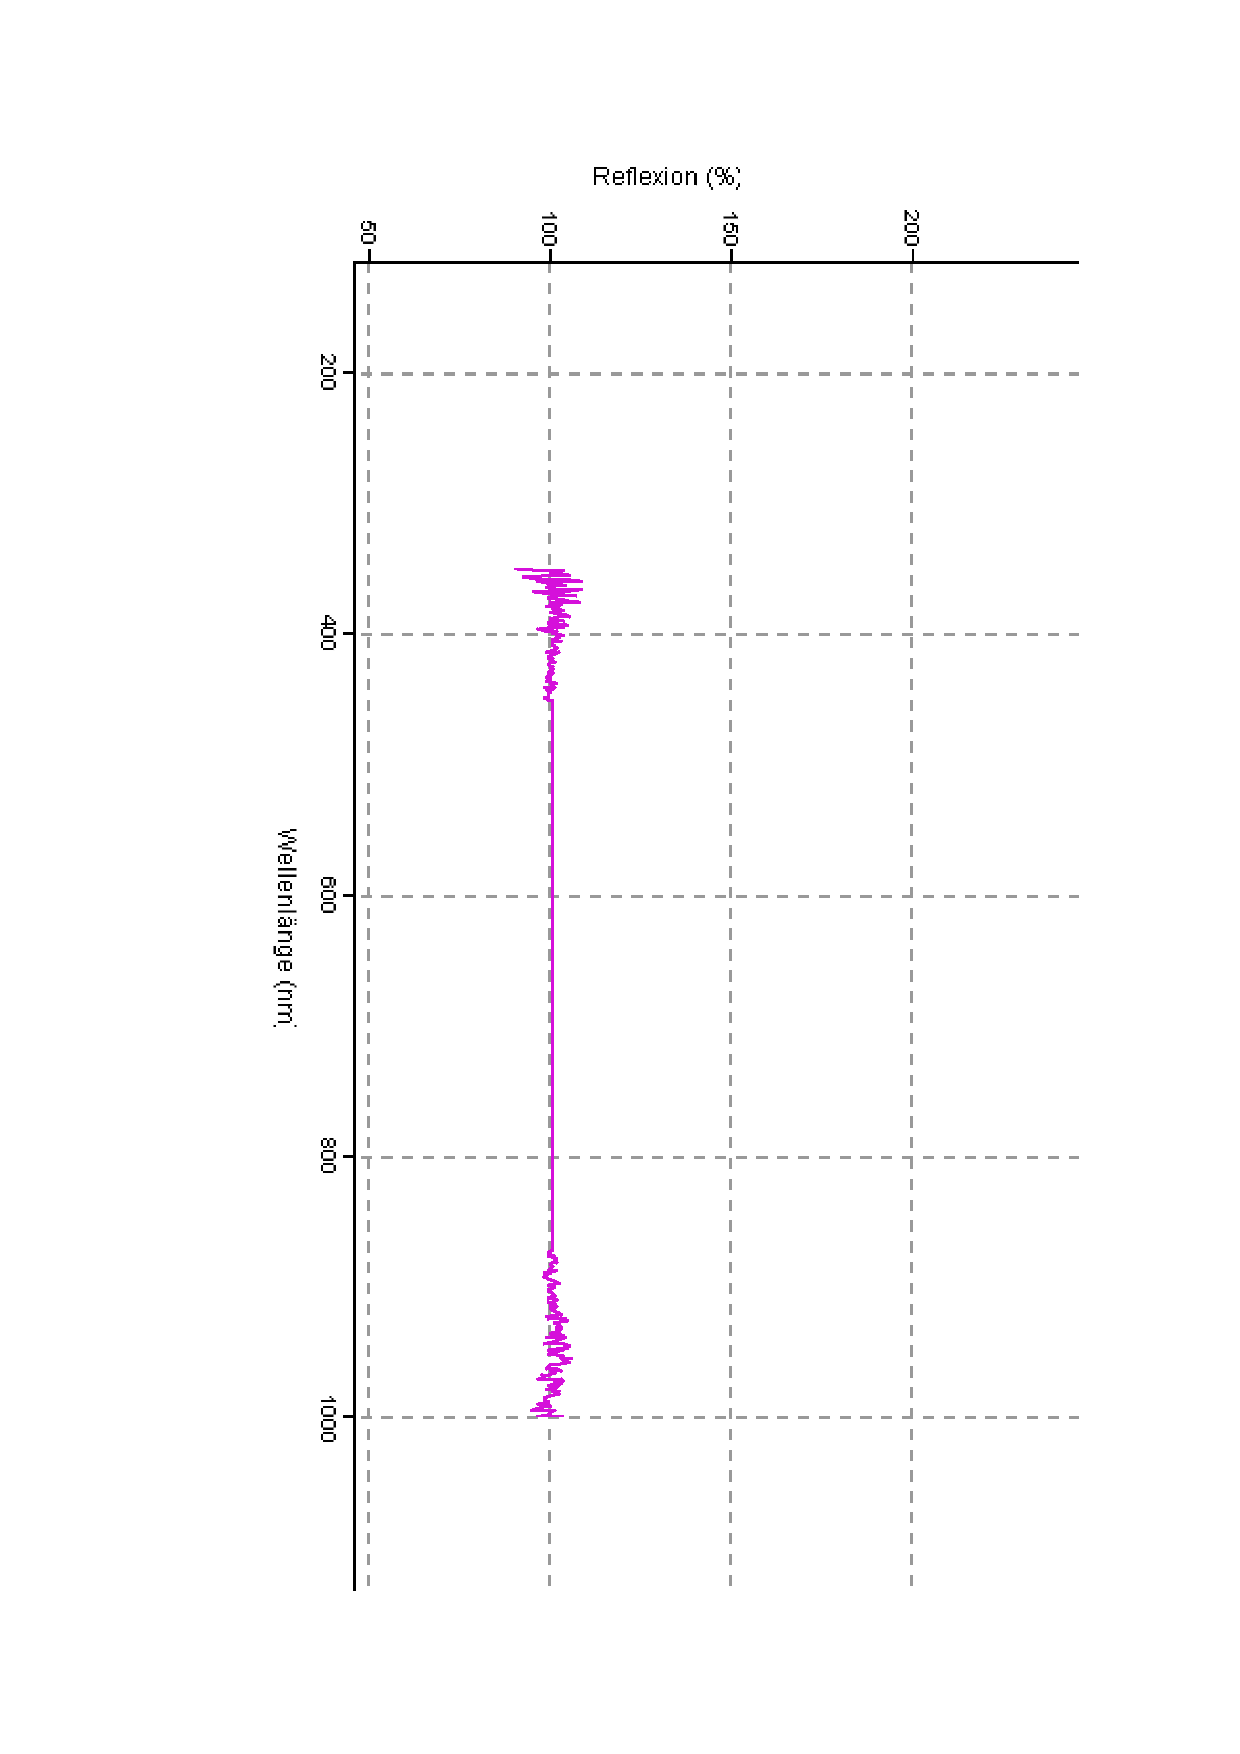
\includegraphics[scale=0.5,angle = 90,trim = 20mm 20mm 20mm 20mm]{./data/Spektro/Interferenzfilter_Leer.pdf}
	\caption{Reflexionsspektrum ohne Interferenzfilter}
	\label{fig:InterferenzOhne}
\end{figure}

\begin{figure}[H]
	\centering
	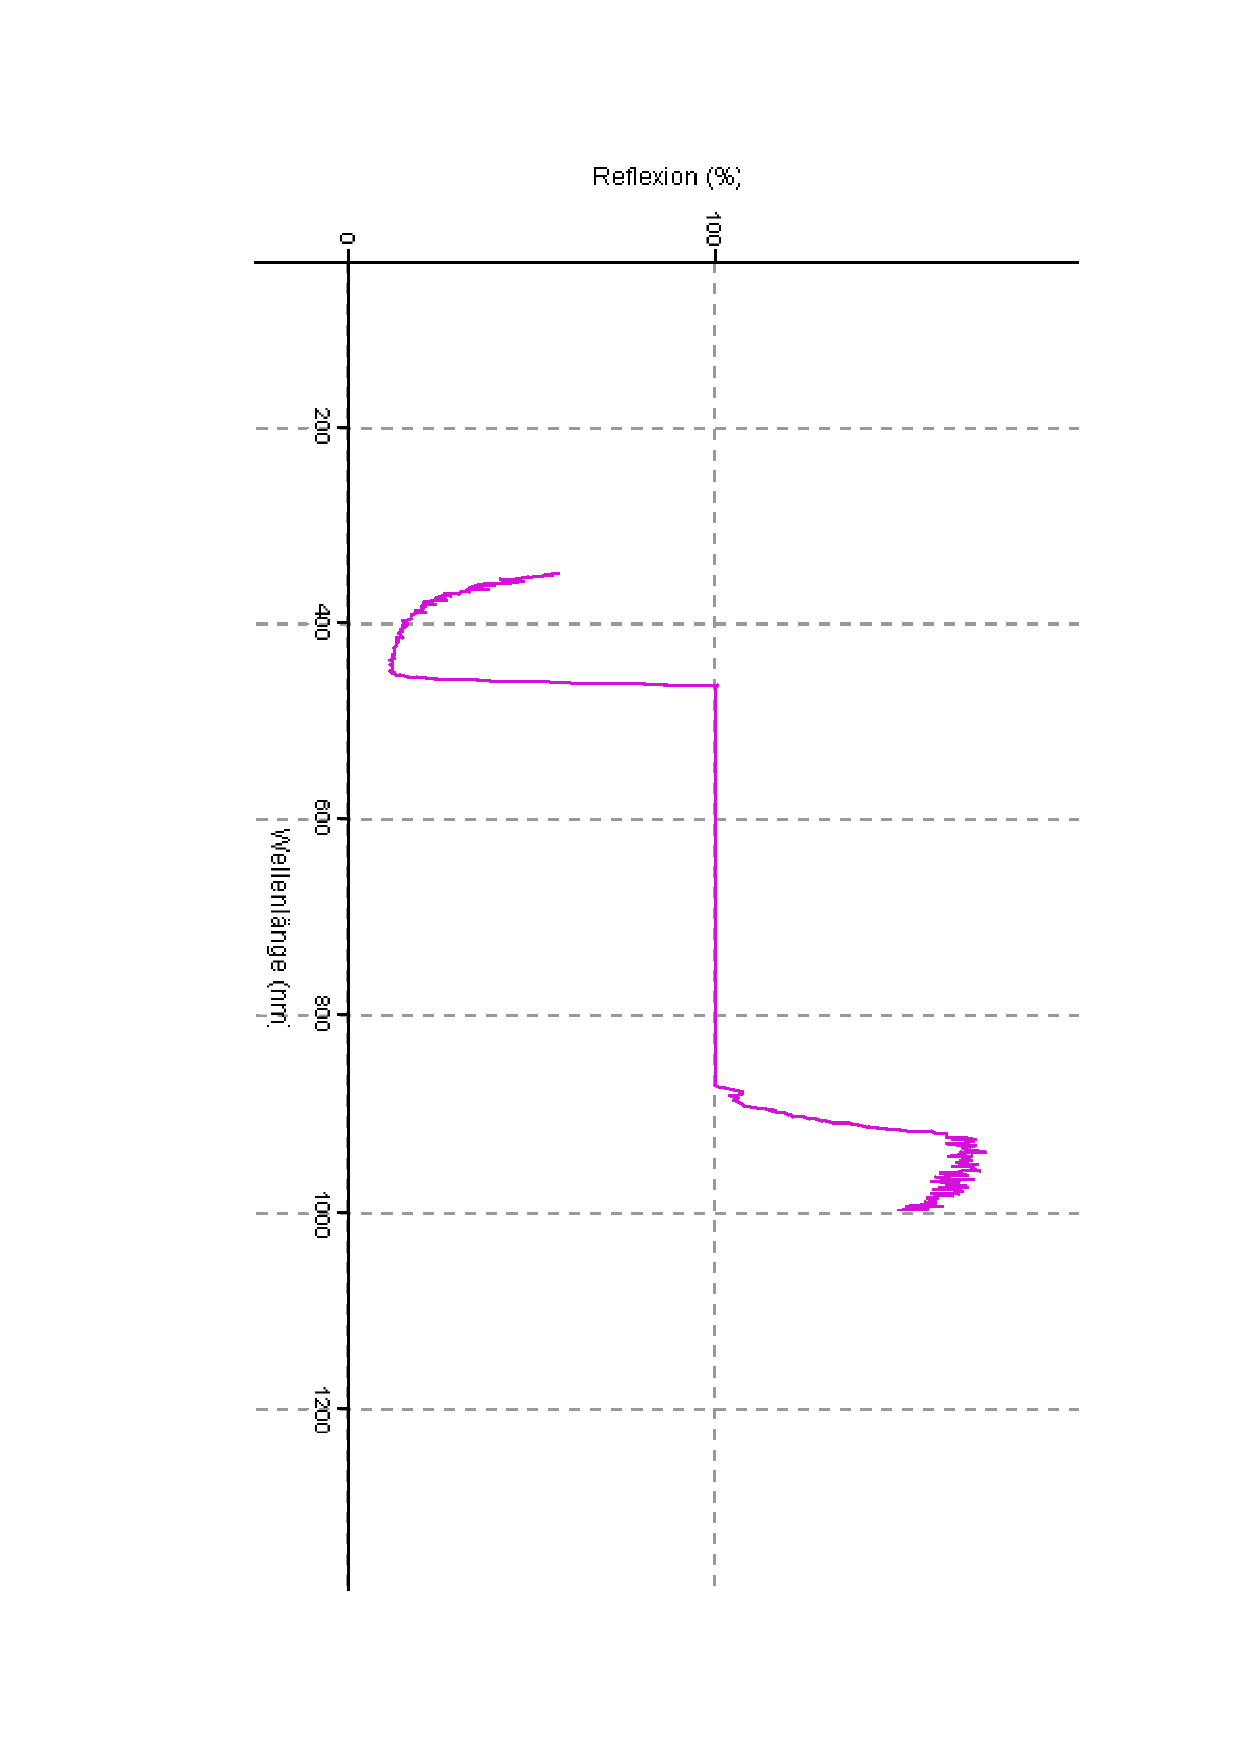
\includegraphics[scale=0.5,angle = 90,trim = 20mm 20mm 20mm 20mm]{./data/Spektro/Interferenzfilter_Gelb.pdf}
	\caption{Reflexionsspektrum mit Interferenzfilter gelbe Seite zugewant}
	\label{fig:InterferenzGelb}
\end{figure}

\begin{figure}[H]
	\centering
	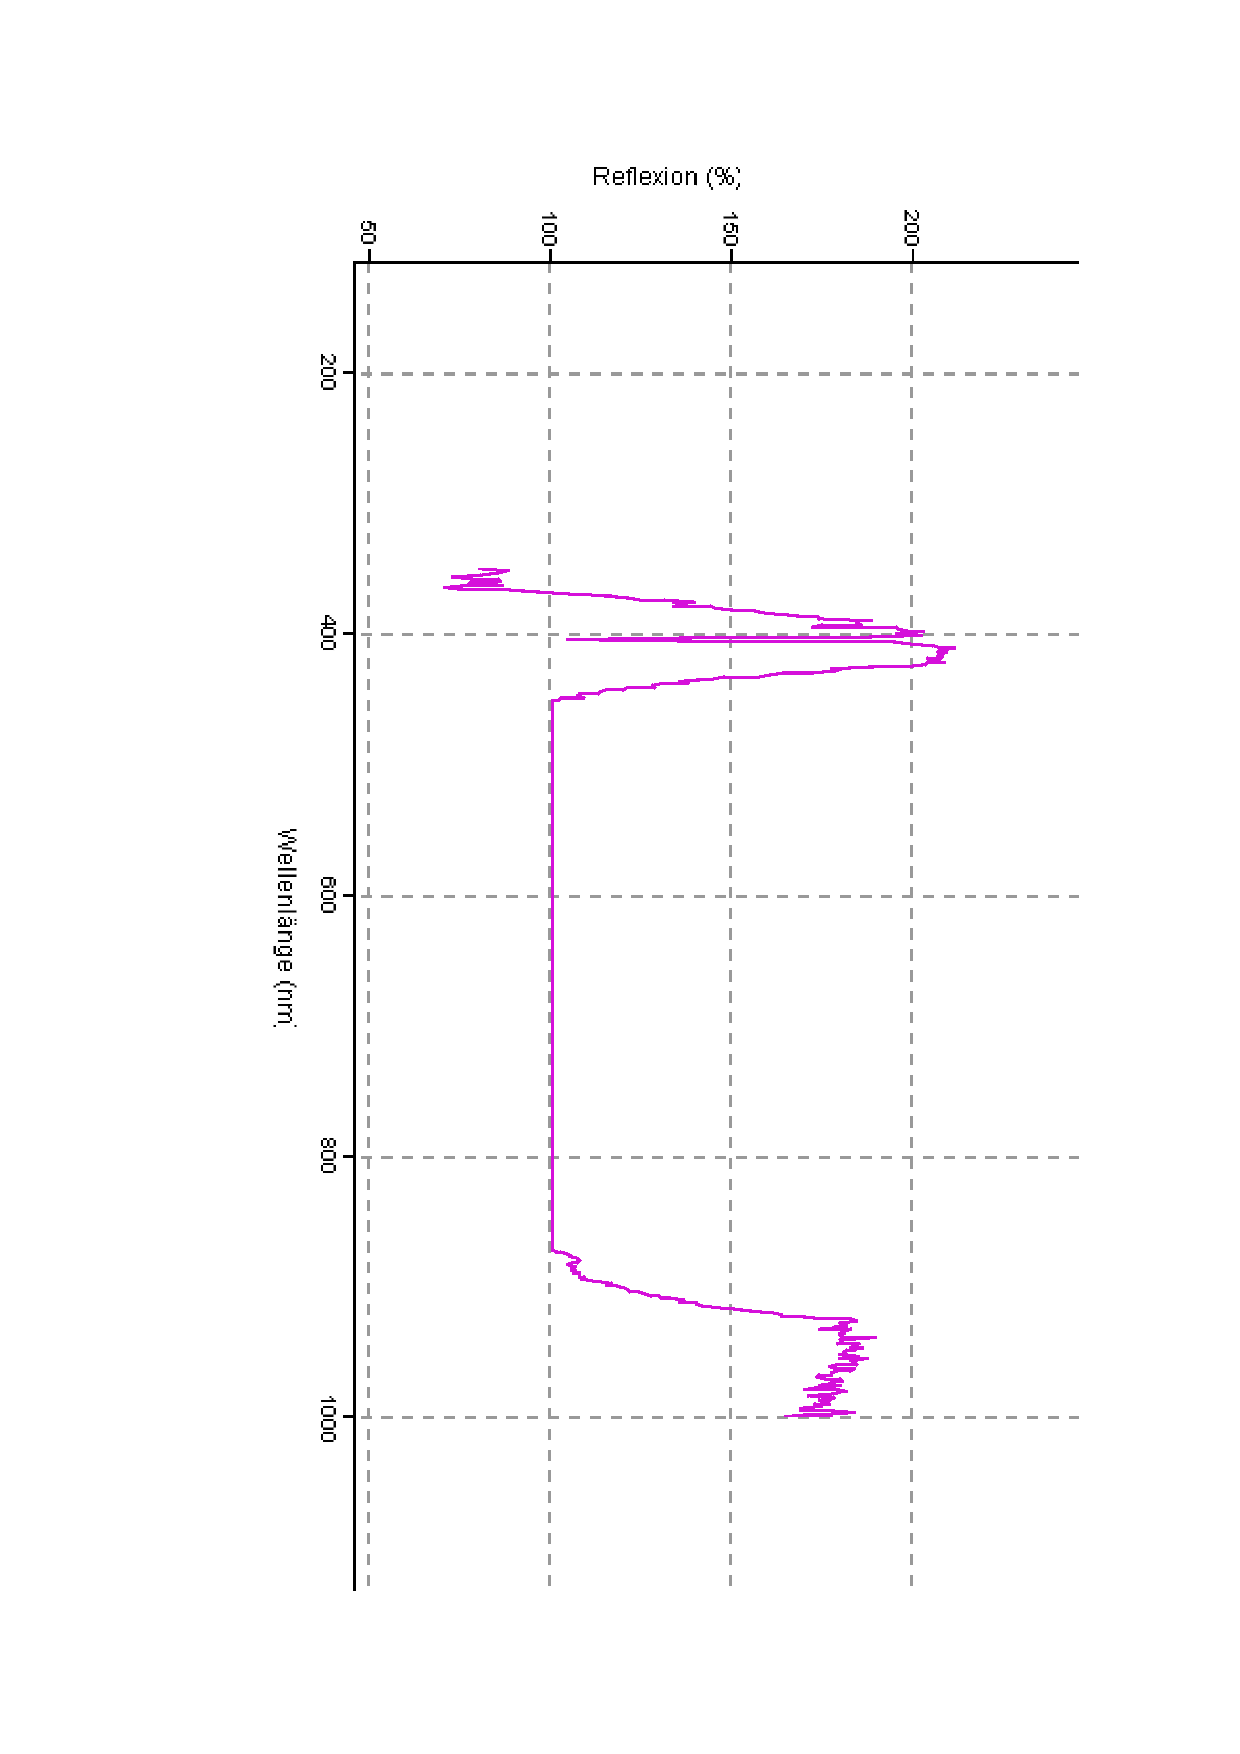
\includegraphics[scale=0.5,angle = 90,trim = 20mm 20mm 20mm 20mm]{./data/Spektro/Interferenzfilter_Silber_480nm.pdf}
	\caption{Reflexionsspektrum mit Interferenzfilter; silberne Seite zugewant}
	\label{fig:InterferenzSilber}
\end{figure}

\begin{figure}[H]
	\centering
	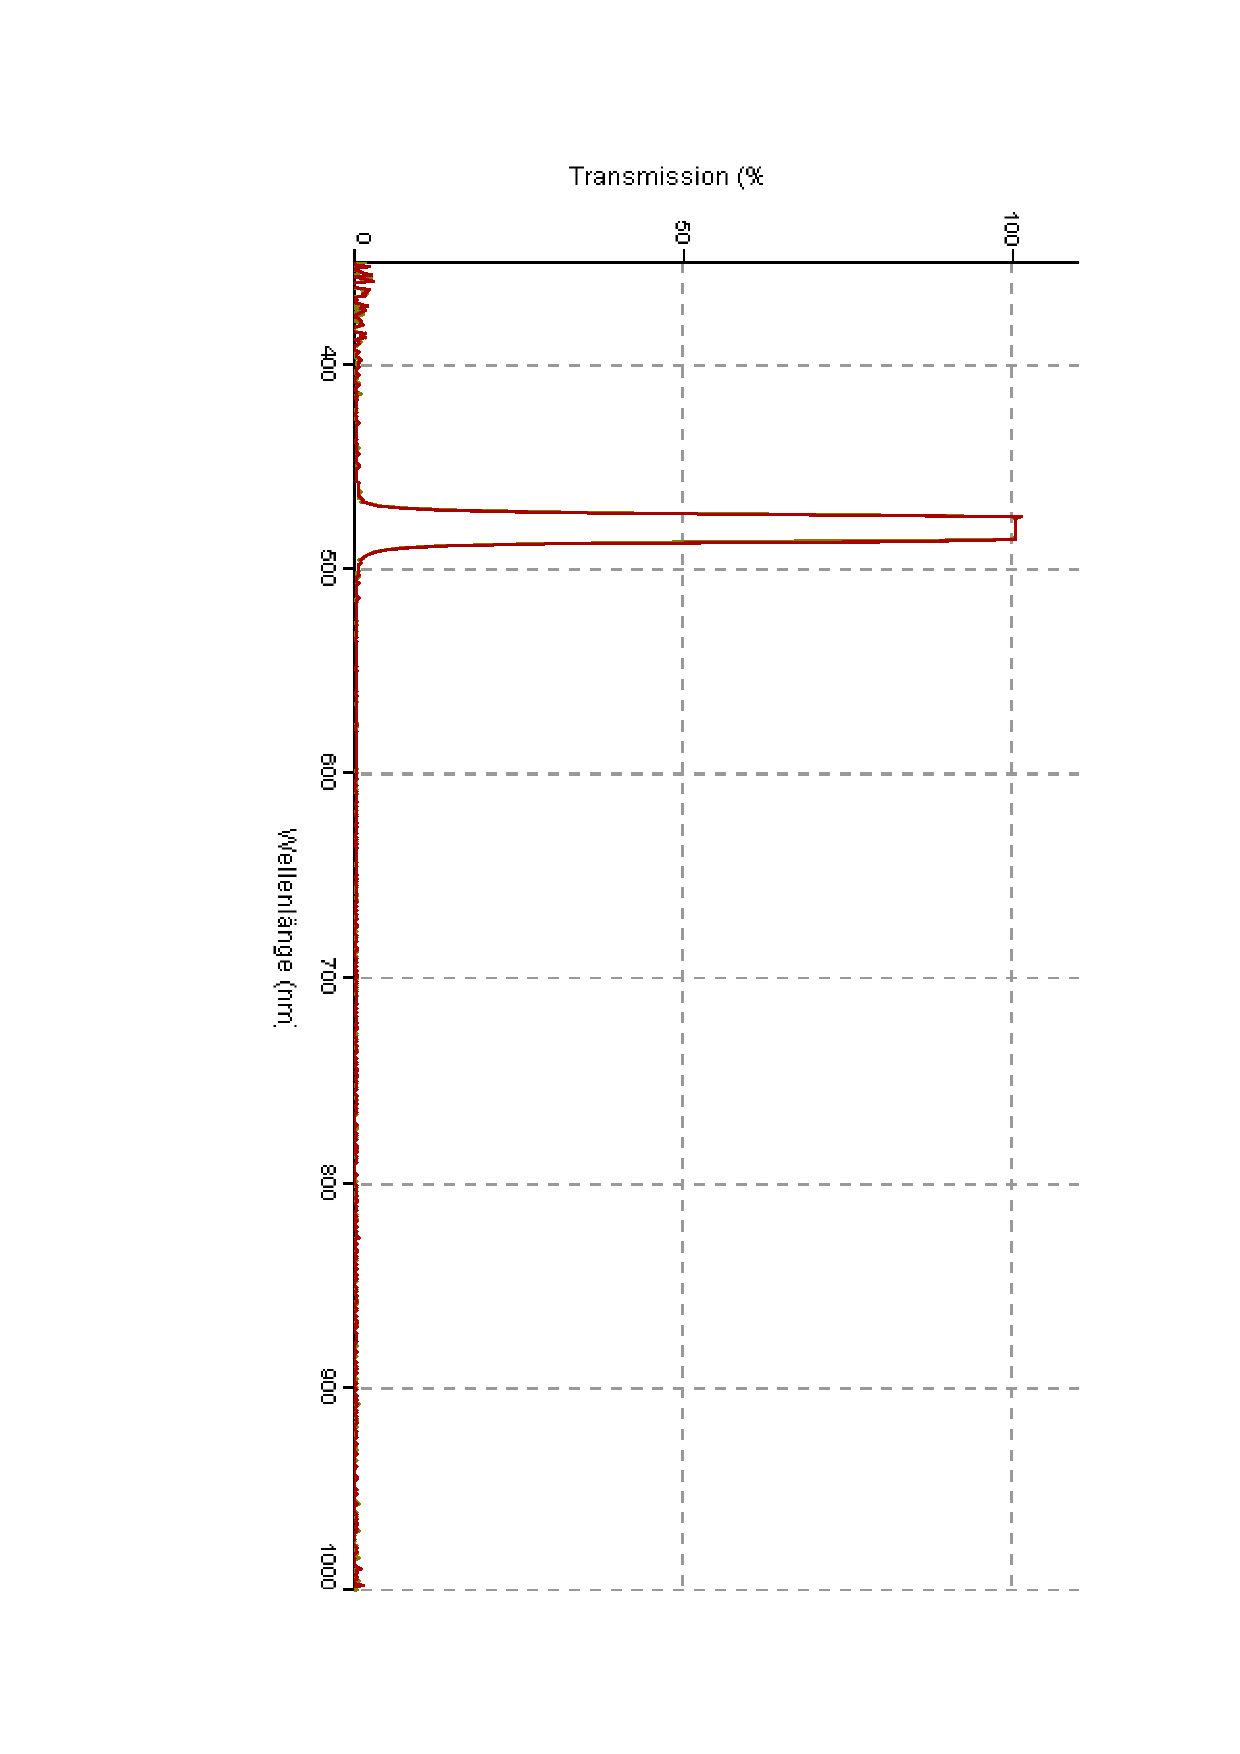
\includegraphics[scale=0.5,angle = 90,trim = 20mm 20mm 20mm 20mm]{./data/Spektro/Interferenzfilter_Transmission_Gelb_Silber.pdf}
	\caption{Transmissionsspektrum mit Interferenzfilter, gelbe und silberne Seite}
	\label{fig:InterferenzSilber}
\end{figure}

\begin{multicols}{2}

\subsection{Michelson-Interferometer}

1. Messung:\\
$N = (100 \pm 1)$ Minima\\
$\Delta l = (31\pm 0.5)\mu m$\\
$$\lambda_1=(620\pm 12)nm$$\\

\noindent 2. Messung:\\
$N=(100 \pm 4)$ Minima\\
$\Delta l = (30 \pm 0.5) \mu m$\\
$$\lambda_2 =(600\pm 41)nm$$\\

\noindent 3. Messung:\\
$N =(100 \pm 5)$ Minima\\
$\Delta l = (28 \pm 0.5)\mu m$\\
$$\lambda_3 = (560\pm 51) nm$$


%%%%%%%%%%%%%%%%%%%%%%%%%%%%%%%%%%%%%%%%%%%%%%%%
%%%%%%%%%%%%%%%%%%%%%%%%%%%%%%%%%%%%%%%%%%%%%%%%
\section{Diskussion}
\subsection{Auflösungsvermögen eines Gitters}

Die Auflösung des Kathetometers beträgt $0.01$ mm, die Unsicherheit für die Messungen der Blendenbreiten wurde jedoch mit $0.05$ mm abgeschätzt. Da sich in Versuchen, die gleiche Breite mehrmals zu messen, aufgrund des Fadenkreuzes und der ausgefransten Spaltenränder, eine gewisse Toleranz der Ergebnisse eingestellt hat, scheint diese eher vorsichtige Abschätzung vernünftig.\\
Würde das Messinstrument öfter verwendet und ein besseres Gefühl für seine Handhabung entwickelt werden, wäre es sicher realistisch, kleinere unsicherheiten (eventuell bis hin zur Auflösung) zuzulassen.\\
\\
Im Kapitel \emph{Resultate} sind die einzelnen Ergebnisse für die Gitterkonstante, an jedem betrachteten Interferenzmaxiumum angegeben, sowie ein gemittelter Wert über alle Ergebnisse.\\
Die Gitterkonstante des verwendeten Gitters wurde also mit \\
$a=(8.82 \pm 0.33)\mu m$\\
bestimmt.\\
Da jedoch die Grenze des Auflösungsvermögens der beiden gelben Spektrallinien in einem gewissen Bereich subjektiv ist, und auch von verschiedenen Umfeldfaktoren abhängt, darf ein wesentlich größerer Unsicherheitsbereich angenommen werden, als der, der sich aus den Messunsicherheiten ergibt.\\
Eine Einschränkung ist die Intensität der betrachteten Linien. Diese ist in der 4. Ordnung ohnehin schon sehr klein, außerdem treten hier die engsten Blendeneinstellungen auf. Dies verringert die Intensität zusätzlich und lässt die Messung sehr schwierig werden. Das zeigt sich auch darin, dass beide Messungen an den Maxima 4. Ordnung die extremsten Ergebnisse darstellen.\\
Aber auch die anderen Messungen sind von momentanen Einflüssen gestört: Da die Blende jeweils abgenommen werden muss, um die Blendenbreite zu bestimmen, wird das Gitter immer wieder bewegt (die Blende wird fest an das Gitter geklemmt). Eine feste Vorrichtung zum Einspannen würde möglicherweise Verbesserungen bringen.\\
Außerdem wurde das Experiment in einem Raum mit einer zweiten Gruppe durchgeführt, die etwas Licht für ihre Arbeit benötigt haben. Auch das ist ein Störeinfluss, der zwar leicht zu beseitigen wäre, aber hier aus praktischen Gründen vorliegt.\\
Es lässt sich also nicht mit Bestimmtheit sagen, dass der wahre Wert innerhalb des Bereiches liegt.\\Nachfragen ergab, dass die Lösung mit $10 \mu m$ angegeben ist. Da jedoch alle Einzelmessungen unter diesem Wert liegen, ist trotz aller Ungenauigkeiten ein systematischer Fehler wahrscheinlich (bzw. eine ungenaue Angabe von Herstellerseite). Dies wäre in erster Näherung zu überprüfen, indem man die Ergebnisse verschiedener Gruppen miteinander vergleicht.\\
\\
Ein einziges Ergebnis liegt über $10\mu m$. Dieses wurde jedoch, vor seiner Berechnung verworfen, da der Messende am Goniometer während der Kathetometermessung unterbrochen hat mit der Begründung, wegen tränender Augen, die Messung am Maximum rechts, 2. Ordnung, wiederholen zu wollen.\\



\subsection{Spektrometrie}
Durch das einfache Messen mit dem Spektrometer konnte die Auswertung sehr genau mit dem Computer durchgeführt werden. \\
Im ersten Beispiel sind die Spektren der beiden Testflüssigkeiten A und B eindeutig zu unterscheiden. Bei A handelt es sich laut Tabelle 1 [1](p. 19) um Praseodym. Zwischen 400nm und 500nm treten die Maxima auf und ein Maximum bei 590. Zu sehen in Abb. \ref{fig:AbsorbtionA} und \ref{fig:TransmissionA}.\\
Bei B handelt es sich um Neodym. Zu erkennen ist dies an den Infrarot-Anteilen bei 800nm und rund 970nm in Abb. \ref{fig:TransmissionB} sowie \ref{fig:AbsorbtionB}.\\
Flüssigkeit C konnte mit Überlagerung vom Spektrum von A (Abb. \ref{fig:AbsorbtionCuA}) und B (Abb. \ref{fig:AbsorbtionCuB}) als Mischung beider Flüssigkeiten identifiziert werden.\\
\\
Bei den Farbfiltern ist der Grüne (Abb. \ref{fig:FilterGruen}) am besten und klarsten abgegrenzt. Der rote Filter (Abb. \ref{fig:FilterRot}) weist über den roten Bereich hinaus noch einen Infrarot-Anteil auf.\\
Am schwächsten ausgeprägt ist der blau/violette Filter (Abb. \ref{fig:FilterBlau}). Grund dafür dürfte sein das das Licht der Quelle in diesem Spektrum nicht mehr die volle Intensität aufweist.\\
\\
Der Interferenzfilter brachte das interessanteste Ergebnis: Reflektiert wurde hauptsächlich der Wellenlängenbereich 900-1000nm. Wellenlängen um 400nm wurden absorbiert (bzw. ausgelöscht), wie in Abb. \ref{fig:InterferenzGelb} zu sehen ist. Wendet man den Filter werden ebenfalls Wellenlängen um 900-1000nm reflektiert und zusätzlich alles bis auf ein Minimum bei 400nm (Abb. \ref{fig:InterferenzSelber}).\\
\\
Bei der Untersuchung der transmittierten Wellenlängen ist klar ein Peak bei 480-490nm zu sehen.\\
Trotz leichtem Rauschen (unter anderem durch Staub und fettigen Fingerabdrücken auf so gut wie allen optischen Bauteilen) waren die Spektren überall unterscheidbar und die Substanzen feststellbar.

\subsection{Michelson-Interferometer}

Die Unsicherheiten der 3 Messungen sind vor allem bestimmt durch die Unsicherheiten der gezählten Minima. Einen großen Effekt auf die Genauigkeit der Messung hätte also ein besserer Zählmodus (automatisiert oder zumindest gefilmt und korrigiert). In dem Bewusstsein wäre auch eine Wiederholung des Experiments mit ausgeruhten Augen (unmittelbar davor Spektroskopie) eine Verbesserung.\\
\\
Die gemessenen Wellenlängen stimmen weitgehend mit der Beschriftung auf dem Laser ($632.8nm$) überein, liegen jedoch generell zu tief. \\
Die Messung 3 deckt als einzige nicht die Herstellerangabe ab, Messung 1 nur knapp.\\
Geht man von einem systematischen Fehler aus (die Alternative, eine falsche Herstellerangabe, kann im Rahmen des Praktikums nicht ausreichend behandelt werden), kann dieser eigentlich nur im Bereich des verstellbaren Spiegels liegen, nicht jedoch in der Kalibrierung der anderen Teile, da ja nur die durchlaufenen Längenunterschiede, nicht jedoch ein absoluter Gangunterschied für die Messung relevant sind.\\
\\
Ausgehend davon, dass die Montage mit Spiegel, Plattform und Mikrometerschraube innerhalb der Auflösung der Mikrometerschraube störungsfrei arbeiten, ist vor allem beim Gummiband und eben vor allem in der Übung mit dem Instrument (also der menschlichen Komponente) nach Verbesserungen zu suchen.


\section{Quellen}
$[1]$ Anleitung, \url{http://www.univie.ac.at/anfpra/neu1/ps/ps4/ps4.pdf}\\
\end{multicols}

\end{document}